\documentclass[twoside]{book}

% Packages required by doxygen
\usepackage{fixltx2e}
\usepackage{calc}
\usepackage{doxygen}
\usepackage[export]{adjustbox} % also loads graphicx
\usepackage{graphicx}
\usepackage[utf8]{inputenc}
\usepackage{makeidx}
\usepackage{multicol}
\usepackage{multirow}
\PassOptionsToPackage{warn}{textcomp}
\usepackage{textcomp}
\usepackage[nointegrals]{wasysym}
\usepackage[table]{xcolor}

% NLS support packages
\usepackage[ngerman]{babel}

% Font selection
\usepackage[T1]{fontenc}
\usepackage[scaled=.90]{helvet}
\usepackage{courier}
\usepackage{amssymb}
\usepackage{sectsty}
\renewcommand{\familydefault}{\sfdefault}
\allsectionsfont{%
  \fontseries{bc}\selectfont%
  \color{darkgray}%
}
\renewcommand{\DoxyLabelFont}{%
  \fontseries{bc}\selectfont%
  \color{darkgray}%
}
\newcommand{\+}{\discretionary{\mbox{\scriptsize$\hookleftarrow$}}{}{}}

% Page & text layout
\usepackage{geometry}
\geometry{%
  a4paper,%
  top=2.5cm,%
  bottom=2.5cm,%
  left=2.5cm,%
  right=2.5cm%
}
\tolerance=750
\hfuzz=15pt
\hbadness=750
\setlength{\emergencystretch}{15pt}
\setlength{\parindent}{0cm}
\setlength{\parskip}{3ex plus 2ex minus 2ex}
\makeatletter
\renewcommand{\paragraph}{%
  \@startsection{paragraph}{4}{0ex}{-1.0ex}{1.0ex}{%
    \normalfont\normalsize\bfseries\SS@parafont%
  }%
}
\renewcommand{\subparagraph}{%
  \@startsection{subparagraph}{5}{0ex}{-1.0ex}{1.0ex}{%
    \normalfont\normalsize\bfseries\SS@subparafont%
  }%
}
\makeatother

% Headers & footers
\usepackage{fancyhdr}
\pagestyle{fancyplain}
\fancyhead[LE]{\fancyplain{}{\bfseries\thepage}}
\fancyhead[CE]{\fancyplain{}{}}
\fancyhead[RE]{\fancyplain{}{\bfseries\leftmark}}
\fancyhead[LO]{\fancyplain{}{\bfseries\rightmark}}
\fancyhead[CO]{\fancyplain{}{}}
\fancyhead[RO]{\fancyplain{}{\bfseries\thepage}}
\fancyfoot[LE]{\fancyplain{}{}}
\fancyfoot[CE]{\fancyplain{}{}}
\fancyfoot[RE]{\fancyplain{}{\bfseries\scriptsize Erzeugt von Doxygen }}
\fancyfoot[LO]{\fancyplain{}{\bfseries\scriptsize Erzeugt von Doxygen }}
\fancyfoot[CO]{\fancyplain{}{}}
\fancyfoot[RO]{\fancyplain{}{}}
\renewcommand{\footrulewidth}{0.4pt}
\renewcommand{\chaptermark}[1]{%
  \markboth{#1}{}%
}
\renewcommand{\sectionmark}[1]{%
  \markright{\thesection\ #1}%
}

% Indices & bibliography
\usepackage{natbib}
\usepackage[titles]{tocloft}
\setcounter{tocdepth}{3}
\setcounter{secnumdepth}{5}
\makeindex

% Hyperlinks (required, but should be loaded last)
\usepackage{ifpdf}
\ifpdf
  \usepackage[pdftex,pagebackref=true]{hyperref}
\else
  \usepackage[ps2pdf,pagebackref=true]{hyperref}
\fi
\hypersetup{%
  colorlinks=true,%
  linkcolor=blue,%
  citecolor=blue,%
  unicode%
}

% Custom commands
\newcommand{\clearemptydoublepage}{%
  \newpage{\pagestyle{empty}\cleardoublepage}%
}

\usepackage{caption}
\captionsetup{labelsep=space,justification=centering,font={bf},singlelinecheck=off,skip=4pt,position=top}

%===== C O N T E N T S =====

\begin{document}

% Titlepage & ToC
\hypersetup{pageanchor=false,
             bookmarksnumbered=true,
             pdfencoding=unicode
            }
\pagenumbering{alph}
\begin{titlepage}
\vspace*{7cm}
\begin{center}%
{\Large V\+H\+DL Switch }\\
\vspace*{1cm}
{\large Erzeugt von Doxygen 1.8.14}\\
\end{center}
\end{titlepage}
\clearemptydoublepage
\pagenumbering{roman}
\tableofcontents
\clearemptydoublepage
\pagenumbering{arabic}
\hypersetup{pageanchor=true}

%--- Begin generated contents ---
\chapter{Design Unit Index}
\section{Design Unit Hierarchy}
Die Liste der Ableitungen ist -\/mit Einschränkungen-\/ alphabetisch sortiert\+:\begin{DoxyCompactList}
\item \contentsline{section}{testbench}{\pageref{classtestbench}}{}
\begin{DoxyCompactList}
\item \contentsline{section}{switch}{\pageref{classswitch}}{}
\end{DoxyCompactList}
\end{DoxyCompactList}

\chapter{Design Unit Index}
\section{Design Unit List}
Here is a list of all design unit members with links to the Entities they belong to\+:\begin{DoxyCompactList}
\item\contentsline{section}{entity \mbox{\hyperlink{classswitch}{switch}} \\*Switch entity Diese Entity implementiert den Switch. Diverse Parameter werden als Generics erst bei der Instanzierung angegeben }{\pageref{classswitch}}{}
\item\contentsline{section}{architecture \mbox{\hyperlink{classswitch_1_1switch}{switch}} \\*Switch architecture In dieser Architecture wird der Switch implementiert }{\pageref{classswitch_1_1switch}}{}
\item\contentsline{section}{entity \mbox{\hyperlink{classtestbench}{testbench}} \\*Testbench entity }{\pageref{classtestbench}}{}
\item\contentsline{section}{architecture \mbox{\hyperlink{classtestbench_1_1testbench}{testbench}} \\*Testbench architecture Mit dieser Testbench wird der Switch getestet. Es werden alle Ausgänge einzeln getestet, sowie ein Broadcast. Ein Paket mit ungültiger Adresse wird ebenfalls getestet, sowie die Funktion des Switch nach einem solchen ungültigen Paket }{\pageref{classtestbench_1_1testbench}}{}
\end{DoxyCompactList}

\chapter{Datei-\/\+Verzeichnis}
\section{Auflistung der Dateien}
Hier folgt die Aufzählung aller dokumentierten Dateien mit einer Kurzbeschreibung\+:\begin{DoxyCompactList}
\item\contentsline{section}{C\+:/fh/fpga/switch/switch.\+srcs/sim\+\_\+1/new/\mbox{\hyperlink{testbench_8vhd}{testbench.\+vhd}} \\*Switch Testbench }{\pageref{testbench_8vhd}}{}
\item\contentsline{section}{C\+:/fh/fpga/switch/switch.\+srcs/sources\+\_\+1/new/\mbox{\hyperlink{constants_8vhd}{constants.\+vhd}} \\*Switch Constants }{\pageref{constants_8vhd}}{}
\item\contentsline{section}{C\+:/fh/fpga/switch/switch.\+srcs/sources\+\_\+1/new/\mbox{\hyperlink{switch_8vhd}{switch.\+vhd}} \\*Switch }{\pageref{switch_8vhd}}{}
\end{DoxyCompactList}

\chapter{Klassen-\/\+Dokumentation}
\hypertarget{classswitch}{}\section{switch Entity Reference}
\label{classswitch}\index{switch@{switch}}


Switch entity Diese Entity implementiert den Switch. Diverse Parameter werden als Generics erst bei der Instanzierung angegeben.  


Klassendiagramm für switch\+:\begin{figure}[H]
\begin{center}
\leavevmode
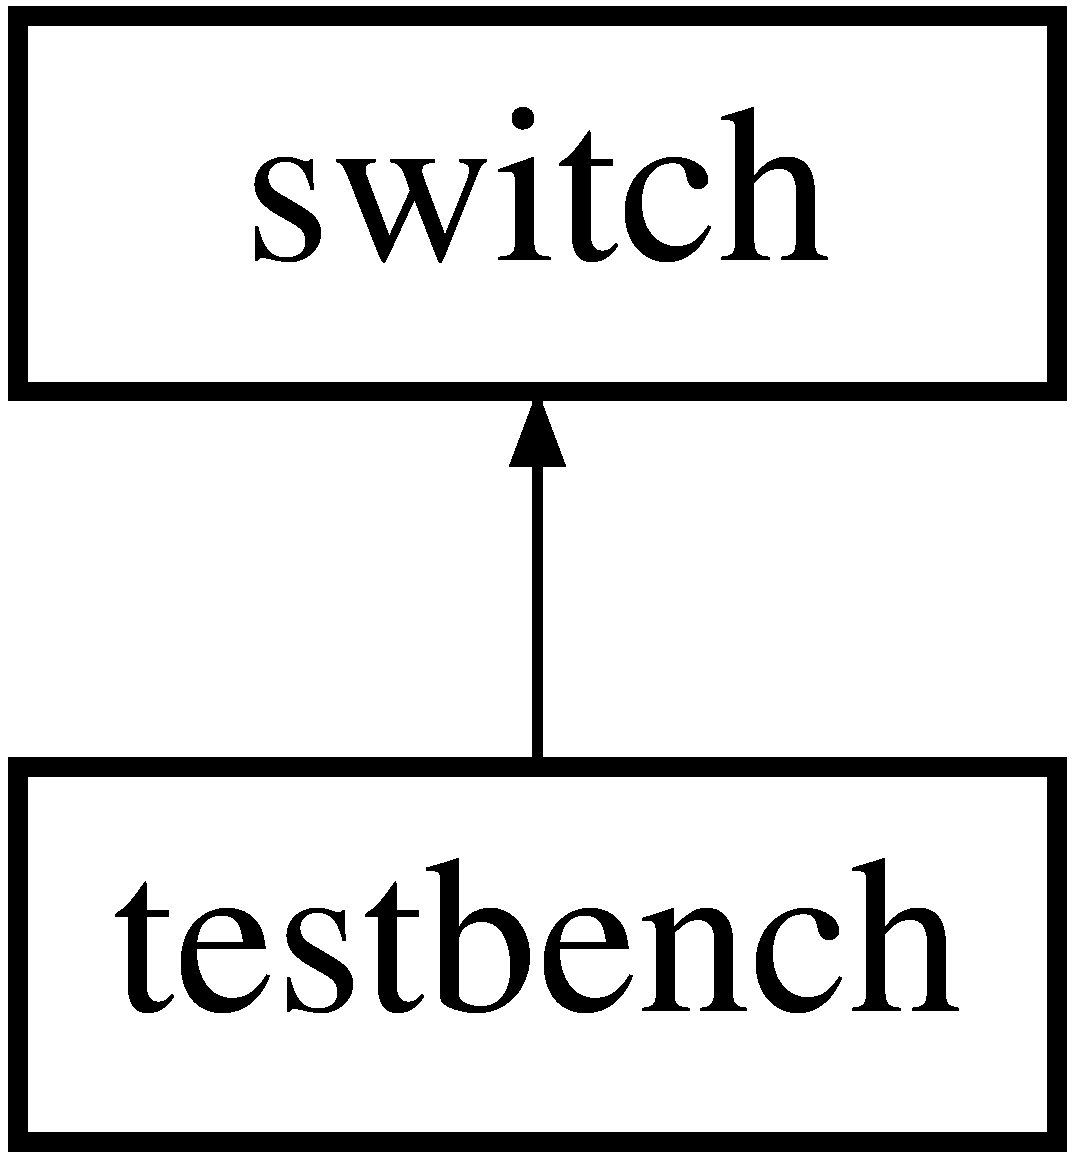
\includegraphics[height=2.000000cm]{classswitch}
\end{center}
\end{figure}
\subsection*{Entities}
\begin{DoxyCompactItemize}
\item 
\mbox{\hyperlink{classswitch_1_1switch}{switch}} architecture
\begin{DoxyCompactList}\small\item\em Switch architecture In dieser Architecture wird der Switch implementiert. \end{DoxyCompactList}\end{DoxyCompactItemize}
\subsection*{Libraries}
 \begin{DoxyCompactItemize}
\item 
\mbox{\Hypertarget{classswitch_ae4f03c286607f3181e16b9aa12d0c6d4}\label{classswitch_ae4f03c286607f3181e16b9aa12d0c6d4}} 
\mbox{\hyperlink{classswitch_ae4f03c286607f3181e16b9aa12d0c6d4}{I\+E\+EE}} 
\begin{DoxyCompactList}\small\item\em Use standard library. \end{DoxyCompactList}\end{DoxyCompactItemize}
\subsection*{Use Clauses}
 \begin{DoxyCompactItemize}
\item 
\mbox{\Hypertarget{classswitch_aa4b2b25246a821511120e3149b003563}\label{classswitch_aa4b2b25246a821511120e3149b003563}} 
\mbox{\hyperlink{classswitch_aa4b2b25246a821511120e3149b003563}{S\+T\+D\+\_\+\+L\+O\+G\+I\+C\+\_\+1164}}   
\begin{DoxyCompactList}\small\item\em Use std\+\_\+lgoic functions. \end{DoxyCompactList}\item 
\mbox{\Hypertarget{classswitch_a46ad374fc1935ff761f9c11bad3a0719}\label{classswitch_a46ad374fc1935ff761f9c11bad3a0719}} 
\mbox{\hyperlink{classswitch_a46ad374fc1935ff761f9c11bad3a0719}{switch\+\_\+constants}}   
\begin{DoxyCompactList}\small\item\em Use constant definitions. \end{DoxyCompactList}\item 
\mbox{\Hypertarget{classswitch_ae00f3f04545af57582ff10609eee23e2}\label{classswitch_ae00f3f04545af57582ff10609eee23e2}} 
\mbox{\hyperlink{classswitch_ae00f3f04545af57582ff10609eee23e2}{N\+U\+M\+E\+R\+I\+C\+\_\+\+S\+TD}}   
\begin{DoxyCompactList}\small\item\em Use numeric functions. \end{DoxyCompactList}\end{DoxyCompactItemize}
\subsection*{Generics}
 \begin{DoxyCompactItemize}
\item 
\mbox{\Hypertarget{classswitch_ac3d29a0b6e2054c99b41ad85df850fa1}\label{classswitch_ac3d29a0b6e2054c99b41ad85df850fa1}} 
\mbox{\hyperlink{classswitch_ac3d29a0b6e2054c99b41ad85df850fa1}{W\+I\+D\+TH}} {\bfseries {\bfseries \textcolor{comment}{integer}\textcolor{vhdlchar}{ }\textcolor{vhdlchar}{ }\textcolor{vhdlchar}{\+:}\textcolor{vhdlchar}{=}\textcolor{vhdlchar}{ }\textcolor{vhdlchar}{ } \textcolor{vhdldigit}{8} \textcolor{vhdlchar}{ }}}
\begin{DoxyCompactList}\small\item\em Wortbreite (parallel) \end{DoxyCompactList}\item 
\mbox{\Hypertarget{classswitch_a83fa8fb9d47549377f34e64e6cb10446}\label{classswitch_a83fa8fb9d47549377f34e64e6cb10446}} 
\mbox{\hyperlink{classswitch_a83fa8fb9d47549377f34e64e6cb10446}{N\+U\+M\+\_\+\+O\+U\+T\+P\+U\+TS}} {\bfseries {\bfseries \textcolor{comment}{integer}\textcolor{vhdlchar}{ }\textcolor{vhdlchar}{ }\textcolor{vhdlchar}{\+:}\textcolor{vhdlchar}{=}\textcolor{vhdlchar}{ }\textcolor{vhdlchar}{ } \textcolor{vhdldigit}{4} \textcolor{vhdlchar}{ }}}
\begin{DoxyCompactList}\small\item\em Anzahl der Ausgänge. \end{DoxyCompactList}\item 
\mbox{\Hypertarget{classswitch_a9471bdd4db653e9a1f455d5147a685c2}\label{classswitch_a9471bdd4db653e9a1f455d5147a685c2}} 
\mbox{\hyperlink{classswitch_a9471bdd4db653e9a1f455d5147a685c2}{P\+K\+T\+\_\+\+L\+EN}} {\bfseries {\bfseries \textcolor{comment}{integer}\textcolor{vhdlchar}{ }\textcolor{vhdlchar}{ }\textcolor{vhdlchar}{\+:}\textcolor{vhdlchar}{=}\textcolor{vhdlchar}{ }\textcolor{vhdlchar}{ } \textcolor{vhdldigit}{20} \textcolor{vhdlchar}{ }}}
\begin{DoxyCompactList}\small\item\em Länge der Datenpakete. \end{DoxyCompactList}\item 
\mbox{\Hypertarget{classswitch_afc0c5f511c854ac6822209338935e527}\label{classswitch_afc0c5f511c854ac6822209338935e527}} 
\mbox{\hyperlink{classswitch_afc0c5f511c854ac6822209338935e527}{P\+A\+U\+S\+E\+\_\+\+L\+EN}} {\bfseries {\bfseries \textcolor{comment}{integer}\textcolor{vhdlchar}{ }\textcolor{vhdlchar}{ }\textcolor{vhdlchar}{\+:}\textcolor{vhdlchar}{=}\textcolor{vhdlchar}{ }\textcolor{vhdlchar}{ } \textcolor{vhdldigit}{10} \textcolor{vhdlchar}{ }}}
\begin{DoxyCompactList}\small\item\em Länge der Pause zwischen Paketen. \end{DoxyCompactList}\end{DoxyCompactItemize}
\subsection*{Ports}
 \begin{DoxyCompactItemize}
\item 
\mbox{\Hypertarget{classswitch_a4a4609c199d30b3adebbeb3a01276ec5}\label{classswitch_a4a4609c199d30b3adebbeb3a01276ec5}} 
\mbox{\hyperlink{classswitch_a4a4609c199d30b3adebbeb3a01276ec5}{clk}}  {\bfseries {\bfseries \textcolor{keywordflow}{in}\textcolor{vhdlchar}{ }}} {\bfseries \textcolor{comment}{std\+\_\+logic}\textcolor{vhdlchar}{ }} 
\begin{DoxyCompactList}\small\item\em Takt. \end{DoxyCompactList}\item 
\mbox{\Hypertarget{classswitch_a2b3987f98197ec2f7358c2e5e91f234e}\label{classswitch_a2b3987f98197ec2f7358c2e5e91f234e}} 
\mbox{\hyperlink{classswitch_a2b3987f98197ec2f7358c2e5e91f234e}{input}}  {\bfseries {\bfseries \textcolor{keywordflow}{in}\textcolor{vhdlchar}{ }}} {\bfseries \textcolor{comment}{std\+\_\+logic\+\_\+vector}\textcolor{vhdlchar}{ }\textcolor{vhdlchar}{(}\textcolor{vhdlchar}{ }\textcolor{vhdlchar}{ }\textcolor{vhdlchar}{ }\textcolor{vhdlchar}{ }{\bfseries \mbox{\hyperlink{classswitch_ac3d29a0b6e2054c99b41ad85df850fa1}{W\+I\+D\+TH}}} \textcolor{vhdlchar}{-\/}\textcolor{vhdlchar}{ } \textcolor{vhdldigit}{1} \textcolor{vhdlchar}{ }\textcolor{keywordflow}{downto}\textcolor{vhdlchar}{ }\textcolor{vhdlchar}{ } \textcolor{vhdldigit}{0} \textcolor{vhdlchar}{ }\textcolor{vhdlchar}{)}\textcolor{vhdlchar}{ }} 
\begin{DoxyCompactList}\small\item\em Eingang. \end{DoxyCompactList}\item 
\mbox{\Hypertarget{classswitch_ad39843cd1c61c04cf486a1276f95c950}\label{classswitch_ad39843cd1c61c04cf486a1276f95c950}} 
\mbox{\hyperlink{classswitch_ad39843cd1c61c04cf486a1276f95c950}{outputs}}  {\bfseries {\bfseries \textcolor{keywordflow}{out}\textcolor{vhdlchar}{ }}} {\bfseries {\bfseries \mbox{\hyperlink{classswitch__constants_ab8800f6bfb13a05fb4b8f9cf70129f9a}{std\+\_\+logic\+\_\+array}}} \textcolor{vhdlchar}{ }\textcolor{vhdlchar}{(}\textcolor{vhdlchar}{ }\textcolor{vhdlchar}{ } \textcolor{vhdldigit}{1} \textcolor{vhdlchar}{ }\textcolor{keywordflow}{to}\textcolor{vhdlchar}{ }\textcolor{vhdlchar}{ }\textcolor{vhdlchar}{ }\textcolor{vhdlchar}{ }{\bfseries \mbox{\hyperlink{classswitch_a83fa8fb9d47549377f34e64e6cb10446}{N\+U\+M\+\_\+\+O\+U\+T\+P\+U\+TS}}} \textcolor{vhdlchar}{ }\textcolor{vhdlchar}{)}\textcolor{vhdlchar}{ }} 
\begin{DoxyCompactList}\small\item\em Array von Ausgängen. \end{DoxyCompactList}\end{DoxyCompactItemize}


\subsection{Ausführliche Beschreibung}
Switch entity Diese Entity implementiert den Switch. Diverse Parameter werden als Generics erst bei der Instanzierung angegeben. 

Definiert in Zeile \mbox{\hyperlink{switch_8vhd_source_l00027}{27}} der Datei \mbox{\hyperlink{switch_8vhd_source}{switch.\+vhd}}.



Die Dokumentation für diese Klasse wurde erzeugt aufgrund der Datei\+:\begin{DoxyCompactItemize}
\item 
C\+:/fh/fpga/switch/switch.\+srcs/sources\+\_\+1/new/\mbox{\hyperlink{switch_8vhd}{switch.\+vhd}}\end{DoxyCompactItemize}

\hypertarget{classswitch_1_1switch}{}\section{switch Architecture Reference}
\label{classswitch_1_1switch}\index{switch@{switch}}


Switch architecture In dieser Architecture wird der Switch implementiert.  


\subsection*{Processes}
 \begin{DoxyCompactItemize}
\item 
\mbox{\Hypertarget{classswitch_1_1switch_a819d62f4f1dd96137802a2fdd9bfb72e}\label{classswitch_1_1switch_a819d62f4f1dd96137802a2fdd9bfb72e}} 
\mbox{\hyperlink{classswitch_1_1switch_a819d62f4f1dd96137802a2fdd9bfb72e}{read\+\_\+start}}{\bfseries  ( {\bfseries {\bfseries \mbox{\hyperlink{classswitch_a2b3987f98197ec2f7358c2e5e91f234e}{input}}} \textcolor{vhdlchar}{ }} , {\bfseries {\bfseries \mbox{\hyperlink{classswitch_a4a4609c199d30b3adebbeb3a01276ec5}{clk}}} \textcolor{vhdlchar}{ }} )}
\begin{DoxyCompactList}\small\item\em read\+\_\+start\+: speichert das erste Byte des Datenpakets als Zieladresse \end{DoxyCompactList}\item 
\mbox{\Hypertarget{classswitch_1_1switch_aeb3ad6373550eeb671e35a9223c001a6}\label{classswitch_1_1switch_aeb3ad6373550eeb671e35a9223c001a6}} 
\mbox{\hyperlink{classswitch_1_1switch_aeb3ad6373550eeb671e35a9223c001a6}{forward}}{\bfseries  ( {\bfseries {\bfseries \mbox{\hyperlink{classswitch_a2b3987f98197ec2f7358c2e5e91f234e}{input}}} \textcolor{vhdlchar}{ }} , {\bfseries {\bfseries \mbox{\hyperlink{classswitch_a4a4609c199d30b3adebbeb3a01276ec5}{clk}}} \textcolor{vhdlchar}{ }} )}
\begin{DoxyCompactList}\small\item\em warten auf neue Daten -\/ Adresse ist erstes Byte, danach wird listen auf false gesetzt \end{DoxyCompactList}\end{DoxyCompactItemize}
\subsection*{Constants}
 \begin{DoxyCompactItemize}
\item 
\mbox{\hyperlink{classswitch_1_1switch_a138ff3d13d23e477480ce8fb57e9eab2}{M\+AX}} {\bfseries \textcolor{comment}{integer}\textcolor{vhdlchar}{ }\textcolor{vhdlchar}{ }\textcolor{vhdlchar}{\+:}\textcolor{vhdlchar}{=}\textcolor{vhdlchar}{ }\textcolor{vhdlchar}{ }\textcolor{vhdlchar}{ }\textcolor{vhdlchar}{ }{\bfseries \mbox{\hyperlink{classswitch_a9471bdd4db653e9a1f455d5147a685c2}{P\+K\+T\+\_\+\+L\+EN}}} \textcolor{vhdlchar}{+}\textcolor{vhdlchar}{ }\textcolor{vhdlchar}{ }\textcolor{vhdlchar}{ }{\bfseries \mbox{\hyperlink{classswitch_afc0c5f511c854ac6822209338935e527}{P\+A\+U\+S\+E\+\_\+\+L\+EN}}} \textcolor{vhdlchar}{-\/}\textcolor{vhdlchar}{ } \textcolor{vhdldigit}{1} \textcolor{vhdlchar}{ }} 
\item 
\mbox{\Hypertarget{classswitch_1_1switch_a431fa12d262243a7ee6a374e578e9936}\label{classswitch_1_1switch_a431fa12d262243a7ee6a374e578e9936}} 
\mbox{\hyperlink{classswitch_1_1switch_a431fa12d262243a7ee6a374e578e9936}{A\+D\+D\+R\+\_\+\+M\+AX}} {\bfseries \textcolor{comment}{integer}\textcolor{vhdlchar}{ }\textcolor{vhdlchar}{ }\textcolor{vhdlchar}{\+:}\textcolor{vhdlchar}{=}\textcolor{vhdlchar}{ }\textcolor{vhdlchar}{ } \textcolor{vhdldigit}{2} \textcolor{vhdlchar}{$\ast$}\textcolor{vhdlchar}{$\ast$}\textcolor{vhdlchar}{ }\textcolor{vhdlchar}{ }\textcolor{vhdlchar}{ }{\bfseries \mbox{\hyperlink{classswitch_ac3d29a0b6e2054c99b41ad85df850fa1}{W\+I\+D\+TH}}} \textcolor{vhdlchar}{-\/}\textcolor{vhdlchar}{ } \textcolor{vhdldigit}{1} \textcolor{vhdlchar}{ }} 
\begin{DoxyCompactList}\small\item\em Broadcast-\/\+Adresse. \end{DoxyCompactList}\end{DoxyCompactItemize}
\subsection*{Signals}
 \begin{DoxyCompactItemize}
\item 
\mbox{\Hypertarget{classswitch_1_1switch_aadc756e11ce964b6d882b33148e05b0d}\label{classswitch_1_1switch_aadc756e11ce964b6d882b33148e05b0d}} 
\mbox{\hyperlink{classswitch_1_1switch_aadc756e11ce964b6d882b33148e05b0d}{finished}} {\bfseries \textcolor{comment}{boolean}\textcolor{vhdlchar}{ }\textcolor{vhdlchar}{ }\textcolor{vhdlchar}{\+:}\textcolor{vhdlchar}{=}\textcolor{vhdlchar}{ }\textcolor{vhdlchar}{ }\textcolor{vhdlchar}{ }\textcolor{vhdlchar}{ }\textcolor{vhdlchar}{false}\textcolor{vhdlchar}{ }} 
\begin{DoxyCompactList}\small\item\em Datenpaket komplett übertragen. \end{DoxyCompactList}\end{DoxyCompactItemize}
\subsection*{Shared Variables}
 \begin{DoxyCompactItemize}
\item 
\mbox{\Hypertarget{classswitch_1_1switch_a5229ed80855aa1ab6c3125663592e274}\label{classswitch_1_1switch_a5229ed80855aa1ab6c3125663592e274}} 
\mbox{\hyperlink{classswitch_1_1switch_a5229ed80855aa1ab6c3125663592e274}{address}} {\bfseries \textcolor{keywordflow}{shared}\textcolor{vhdlchar}{ }\textcolor{comment}{integer}\textcolor{vhdlchar}{ }\textcolor{vhdlchar}{ }\textcolor{vhdlchar}{ }\textcolor{keywordflow}{range}\textcolor{vhdlchar}{ }\textcolor{vhdlchar}{ } \textcolor{vhdldigit}{0} \textcolor{vhdlchar}{ }\textcolor{keywordflow}{to}\textcolor{vhdlchar}{ }\textcolor{vhdlchar}{(}\textcolor{vhdlchar}{ }\textcolor{vhdlchar}{(}\textcolor{vhdlchar}{ }\textcolor{vhdlchar}{ } \textcolor{vhdldigit}{2} \textcolor{vhdlchar}{$\ast$}\textcolor{vhdlchar}{$\ast$}\textcolor{vhdlchar}{ }\textcolor{vhdlchar}{ }\textcolor{vhdlchar}{ }{\bfseries \mbox{\hyperlink{classswitch_a2b3987f98197ec2f7358c2e5e91f234e}{input}}} \textcolor{vhdlchar}{ }\textcolor{vhdlchar}{\textquotesingle{}}\textcolor{vhdlchar}{ }\textcolor{vhdlkeyword}{length}\textcolor{vhdlchar}{ }\textcolor{vhdlchar}{)}\textcolor{vhdlchar}{ }\textcolor{vhdlchar}{-\/}\textcolor{vhdlchar}{ } \textcolor{vhdldigit}{1} \textcolor{vhdlchar}{ }\textcolor{vhdlchar}{)}\textcolor{vhdlchar}{ }} 
\begin{DoxyCompactList}\small\item\em Adresse -\/ mögliche Werte\+: 0 to 255 (für W\+I\+D\+TH=8) \end{DoxyCompactList}\end{DoxyCompactItemize}


\subsection{Ausführliche Beschreibung}
Switch architecture In dieser Architecture wird der Switch implementiert. 

Definiert in Zeile \mbox{\hyperlink{switch_8vhd_source_l00044}{44}} der Datei \mbox{\hyperlink{switch_8vhd_source}{switch.\+vhd}}.



\subsection{Dokumentation der Datenelemente}
\mbox{\Hypertarget{classswitch_1_1switch_a138ff3d13d23e477480ce8fb57e9eab2}\label{classswitch_1_1switch_a138ff3d13d23e477480ce8fb57e9eab2}} 
\index{switch\+::switch@{switch\+::switch}!M\+AX@{M\+AX}}
\index{M\+AX@{M\+AX}!switch\+::switch@{switch\+::switch}}
\subsubsection{\texorpdfstring{M\+AX}{MAX}}
{\footnotesize\ttfamily \mbox{\hyperlink{classswitch_1_1switch_a138ff3d13d23e477480ce8fb57e9eab2}{M\+AX}} {\bfseries \textcolor{comment}{integer}\textcolor{vhdlchar}{ }\textcolor{vhdlchar}{ }\textcolor{vhdlchar}{\+:}\textcolor{vhdlchar}{=}\textcolor{vhdlchar}{ }\textcolor{vhdlchar}{ }\textcolor{vhdlchar}{ }\textcolor{vhdlchar}{ }{\bfseries \mbox{\hyperlink{classswitch_a9471bdd4db653e9a1f455d5147a685c2}{P\+K\+T\+\_\+\+L\+EN}}} \textcolor{vhdlchar}{+}\textcolor{vhdlchar}{ }\textcolor{vhdlchar}{ }\textcolor{vhdlchar}{ }{\bfseries \mbox{\hyperlink{classswitch_afc0c5f511c854ac6822209338935e527}{P\+A\+U\+S\+E\+\_\+\+L\+EN}}} \textcolor{vhdlchar}{-\/}\textcolor{vhdlchar}{ } \textcolor{vhdldigit}{1} \textcolor{vhdlchar}{ }} \hspace{0.3cm}{\ttfamily [Constant]}}

Länge von Datenpaket + Pause -\/ 1\+: 20 + 10 -\/ 1 = 29 Bytes 1 Takt Abzug wegen Handshake über signal finished 

Definiert in Zeile \mbox{\hyperlink{switch_8vhd_source_l00049}{49}} der Datei \mbox{\hyperlink{switch_8vhd_source}{switch.\+vhd}}.



Die Dokumentation für diese Klasse wurde erzeugt aufgrund der Datei\+:\begin{DoxyCompactItemize}
\item 
C\+:/fh/fpga/switch/switch.\+srcs/sources\+\_\+1/new/\mbox{\hyperlink{switch_8vhd}{switch.\+vhd}}\end{DoxyCompactItemize}

\hypertarget{classswitch__constants}{}\section{switch\+\_\+constants Package Reference}
\label{classswitch__constants}\index{switch\+\_\+constants@{switch\+\_\+constants}}
\subsection*{Libraries}
 \begin{DoxyCompactItemize}
\item 
\mbox{\Hypertarget{classswitch__constants_ae4f03c286607f3181e16b9aa12d0c6d4}\label{classswitch__constants_ae4f03c286607f3181e16b9aa12d0c6d4}} 
\mbox{\hyperlink{classswitch__constants_ae4f03c286607f3181e16b9aa12d0c6d4}{I\+E\+EE}} 
\end{DoxyCompactItemize}
\subsection*{Use Clauses}
 \begin{DoxyCompactItemize}
\item 
\mbox{\Hypertarget{classswitch__constants_aa4b2b25246a821511120e3149b003563}\label{classswitch__constants_aa4b2b25246a821511120e3149b003563}} 
\mbox{\hyperlink{classswitch__constants_aa4b2b25246a821511120e3149b003563}{S\+T\+D\+\_\+\+L\+O\+G\+I\+C\+\_\+1164}}   
\end{DoxyCompactItemize}
\subsection*{Constants}
 \begin{DoxyCompactItemize}
\item 
\mbox{\Hypertarget{classswitch__constants_a5d5b54efad1e67dd67aa312c28ef5cae}\label{classswitch__constants_a5d5b54efad1e67dd67aa312c28ef5cae}} 
\mbox{\hyperlink{classswitch__constants_a5d5b54efad1e67dd67aa312c28ef5cae}{N\+U\+M\+\_\+\+O\+U\+T\+P\+U\+TS}} {\bfseries \textcolor{comment}{integer}\textcolor{vhdlchar}{ }\textcolor{vhdlchar}{ }\textcolor{vhdlchar}{\+:}\textcolor{vhdlchar}{=}\textcolor{vhdlchar}{ }\textcolor{vhdlchar}{ } \textcolor{vhdldigit}{4} \textcolor{vhdlchar}{ }} 
\begin{DoxyCompactList}\small\item\em Anzahl der Ausgänge. \end{DoxyCompactList}\item 
\mbox{\Hypertarget{classswitch__constants_a61f3545de1fd97e083485647537d2a2d}\label{classswitch__constants_a61f3545de1fd97e083485647537d2a2d}} 
\mbox{\hyperlink{classswitch__constants_a61f3545de1fd97e083485647537d2a2d}{W\+I\+D\+TH}} {\bfseries \textcolor{comment}{integer}\textcolor{vhdlchar}{ }\textcolor{vhdlchar}{ }\textcolor{vhdlchar}{\+:}\textcolor{vhdlchar}{=}\textcolor{vhdlchar}{ }\textcolor{vhdlchar}{ } \textcolor{vhdldigit}{8} \textcolor{vhdlchar}{ }} 
\begin{DoxyCompactList}\small\item\em Wortbreite. \end{DoxyCompactList}\item 
\mbox{\Hypertarget{classswitch__constants_a13406e763e8cb4595ff53ddecd6c40f2}\label{classswitch__constants_a13406e763e8cb4595ff53ddecd6c40f2}} 
\mbox{\hyperlink{classswitch__constants_a13406e763e8cb4595ff53ddecd6c40f2}{P\+K\+T\+\_\+\+L\+EN}} {\bfseries \textcolor{comment}{integer}\textcolor{vhdlchar}{ }\textcolor{vhdlchar}{ }\textcolor{vhdlchar}{\+:}\textcolor{vhdlchar}{=}\textcolor{vhdlchar}{ }\textcolor{vhdlchar}{ } \textcolor{vhdldigit}{20} \textcolor{vhdlchar}{ }} 
\begin{DoxyCompactList}\small\item\em Länge der Datenpakete. \end{DoxyCompactList}\item 
\mbox{\Hypertarget{classswitch__constants_a15a8d4adaa5b58dfc565f1accbac8505}\label{classswitch__constants_a15a8d4adaa5b58dfc565f1accbac8505}} 
\mbox{\hyperlink{classswitch__constants_a15a8d4adaa5b58dfc565f1accbac8505}{P\+A\+U\+S\+E\+\_\+\+L\+EN}} {\bfseries \textcolor{comment}{integer}\textcolor{vhdlchar}{ }\textcolor{vhdlchar}{ }\textcolor{vhdlchar}{\+:}\textcolor{vhdlchar}{=}\textcolor{vhdlchar}{ }\textcolor{vhdlchar}{ } \textcolor{vhdldigit}{10} \textcolor{vhdlchar}{ }} 
\begin{DoxyCompactList}\small\item\em Länge der Pause. \end{DoxyCompactList}\end{DoxyCompactItemize}
\subsection*{Types}
 \begin{DoxyCompactItemize}
\item 
\mbox{\Hypertarget{classswitch__constants_ab8800f6bfb13a05fb4b8f9cf70129f9a}\label{classswitch__constants_ab8800f6bfb13a05fb4b8f9cf70129f9a}} 
{\bfseries \mbox{\hyperlink{classswitch__constants_ab8800f6bfb13a05fb4b8f9cf70129f9a}{std\+\_\+logic\+\_\+array}}{\bfseries \textcolor{keywordflow}{array}\textcolor{vhdlchar}{ }\textcolor{vhdlchar}{(}\textcolor{vhdlchar}{ }\textcolor{vhdlchar}{positive}\textcolor{vhdlchar}{ }\textcolor{keywordflow}{range}\textcolor{vhdlchar}{ }\textcolor{vhdlchar}{$<$$>$}\textcolor{vhdlchar}{ }\textcolor{vhdlchar}{)}\textcolor{vhdlchar}{ }\textcolor{vhdlchar}{ }\textcolor{keywordflow}{of}\textcolor{vhdlchar}{ }\textcolor{comment}{std\+\_\+logic\+\_\+vector}\textcolor{vhdlchar}{ }\textcolor{vhdlchar}{(}\textcolor{vhdlchar}{ }\textcolor{vhdlchar}{ }\textcolor{vhdlchar}{ }\textcolor{vhdlchar}{ }{\bfseries \mbox{\hyperlink{classswitch__constants_a61f3545de1fd97e083485647537d2a2d}{W\+I\+D\+TH}}} \textcolor{vhdlchar}{-\/}\textcolor{vhdlchar}{ } \textcolor{vhdldigit}{1} \textcolor{vhdlchar}{ }\textcolor{keywordflow}{downto}\textcolor{vhdlchar}{ }\textcolor{vhdlchar}{ } \textcolor{vhdldigit}{0} \textcolor{vhdlchar}{ }\textcolor{vhdlchar}{)}\textcolor{vhdlchar}{ }}} 
\begin{DoxyCompactList}\small\item\em Array von std\+\_\+logic\+\_\+vector. \end{DoxyCompactList}\end{DoxyCompactItemize}


\subsection{Ausführliche Beschreibung}


Definiert in Zeile \mbox{\hyperlink{constants_8vhd_source_l00013}{13}} der Datei \mbox{\hyperlink{constants_8vhd_source}{constants.\+vhd}}.



Die Dokumentation für diese Klasse wurde erzeugt aufgrund der Datei\+:\begin{DoxyCompactItemize}
\item 
C\+:/fh/fpga/switch/switch.\+srcs/sources\+\_\+1/new/\mbox{\hyperlink{constants_8vhd}{constants.\+vhd}}\end{DoxyCompactItemize}

\hypertarget{classtestbench}{}\section{testbench Entity Reference}
\label{classtestbench}\index{testbench@{testbench}}


Testbench entity.  


Klassendiagramm für testbench\+:\begin{figure}[H]
\begin{center}
\leavevmode
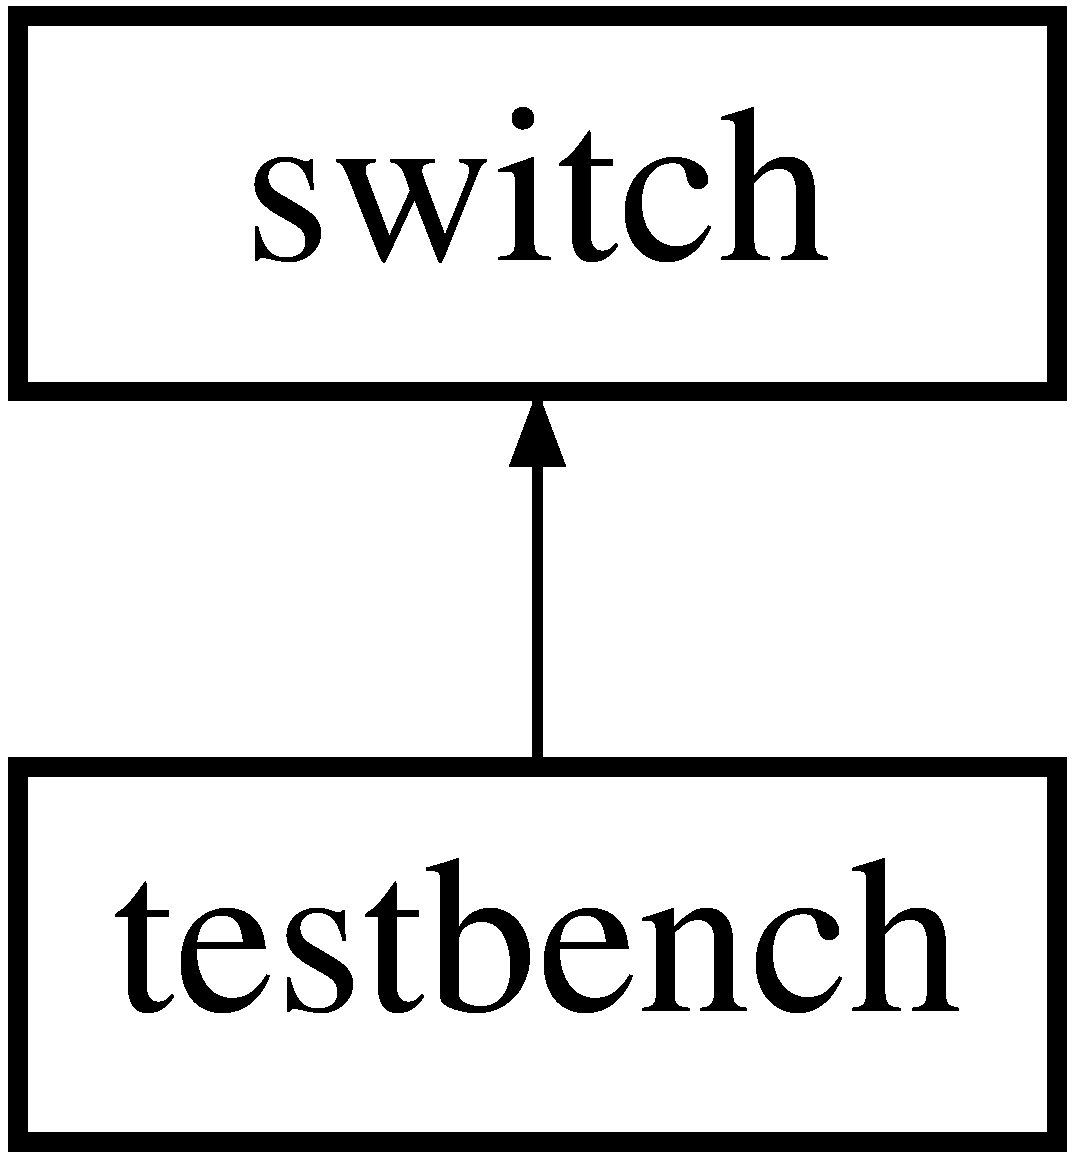
\includegraphics[height=2.000000cm]{classtestbench}
\end{center}
\end{figure}
\subsection*{Entities}
\begin{DoxyCompactItemize}
\item 
\mbox{\hyperlink{classtestbench_1_1testbench}{testbench}} architecture
\begin{DoxyCompactList}\small\item\em Testbench architecture Mit dieser Testbench wird der Switch getestet. Es werden alle Ausgänge einzeln getestet, sowie ein Broadcast. Ein Paket mit ungültiger Adresse wird ebenfalls getestet, sowie die Funktion des Switch nach einem solchen ungültigen Paket. \end{DoxyCompactList}\end{DoxyCompactItemize}
\subsection*{Libraries}
 \begin{DoxyCompactItemize}
\item 
\mbox{\Hypertarget{classtestbench_ae4f03c286607f3181e16b9aa12d0c6d4}\label{classtestbench_ae4f03c286607f3181e16b9aa12d0c6d4}} 
\mbox{\hyperlink{classtestbench_ae4f03c286607f3181e16b9aa12d0c6d4}{I\+E\+EE}} 
\begin{DoxyCompactList}\small\item\em Use standard library. \end{DoxyCompactList}\end{DoxyCompactItemize}
\subsection*{Use Clauses}
 \begin{DoxyCompactItemize}
\item 
\mbox{\Hypertarget{classtestbench_aa4b2b25246a821511120e3149b003563}\label{classtestbench_aa4b2b25246a821511120e3149b003563}} 
\mbox{\hyperlink{classtestbench_aa4b2b25246a821511120e3149b003563}{S\+T\+D\+\_\+\+L\+O\+G\+I\+C\+\_\+1164}}   
\begin{DoxyCompactList}\small\item\em Use std\+\_\+lgoic functions. \end{DoxyCompactList}\item 
\mbox{\Hypertarget{classtestbench_a241c3e72dd8024cc8ae831b1b2aed7db}\label{classtestbench_a241c3e72dd8024cc8ae831b1b2aed7db}} 
\mbox{\hyperlink{classtestbench_a241c3e72dd8024cc8ae831b1b2aed7db}{S\+T\+D\+\_\+\+L\+O\+G\+I\+C\+\_\+\+U\+N\+S\+I\+G\+N\+ED}}   
\begin{DoxyCompactList}\small\item\em Use unsigned logic functions. \end{DoxyCompactList}\item 
\mbox{\Hypertarget{classtestbench_a2edc34402b573437d5f25fa90ba4013e}\label{classtestbench_a2edc34402b573437d5f25fa90ba4013e}} 
\mbox{\hyperlink{classtestbench_a2edc34402b573437d5f25fa90ba4013e}{numeric\+\_\+std}}   
\begin{DoxyCompactList}\small\item\em Use numeric functions. \end{DoxyCompactList}\item 
\mbox{\Hypertarget{classtestbench_a46ad374fc1935ff761f9c11bad3a0719}\label{classtestbench_a46ad374fc1935ff761f9c11bad3a0719}} 
\mbox{\hyperlink{classtestbench_a46ad374fc1935ff761f9c11bad3a0719}{switch\+\_\+constants}}   
\begin{DoxyCompactList}\small\item\em Use constant definitions. \end{DoxyCompactList}\end{DoxyCompactItemize}


\subsection{Ausführliche Beschreibung}
Testbench entity. 

Definiert in Zeile \mbox{\hyperlink{testbench_8vhd_source_l00022}{22}} der Datei \mbox{\hyperlink{testbench_8vhd_source}{testbench.\+vhd}}.



Die Dokumentation für diese Klasse wurde erzeugt aufgrund der Datei\+:\begin{DoxyCompactItemize}
\item 
C\+:/fh/fpga/switch/switch.\+srcs/sim\+\_\+1/new/\mbox{\hyperlink{testbench_8vhd}{testbench.\+vhd}}\end{DoxyCompactItemize}

\hypertarget{classtestbench_1_1testbench}{}\section{testbench Architecture Reference}
\label{classtestbench_1_1testbench}\index{testbench@{testbench}}


Testbench architecture Mit dieser Testbench wird der Switch getestet. Es werden alle Ausgänge einzeln getestet, sowie ein Broadcast. Ein Paket mit ungültiger Adresse wird ebenfalls getestet, sowie die Funktion des Switch nach einem solchen ungültigen Paket.  


\subsection*{Processes}
 \begin{DoxyCompactItemize}
\item 
\mbox{\Hypertarget{classtestbench_1_1testbench_a5e2335f6f6f0aa05413a0546a550ba71}\label{classtestbench_1_1testbench_a5e2335f6f6f0aa05413a0546a550ba71}} 
\mbox{\hyperlink{classtestbench_1_1testbench_a5e2335f6f6f0aa05413a0546a550ba71}{osc}}{\bfseries  (  )}
\begin{DoxyCompactList}\small\item\em osc\+: Taktgenerator \end{DoxyCompactList}\item 
\mbox{\Hypertarget{classtestbench_1_1testbench_a77eeaf075b0fe111c4550ccc6850feb4}\label{classtestbench_1_1testbench_a77eeaf075b0fe111c4550ccc6850feb4}} 
\mbox{\hyperlink{classtestbench_1_1testbench_a77eeaf075b0fe111c4550ccc6850feb4}{Waveforms}}{\bfseries  (  )}
\begin{DoxyCompactList}\small\item\em Waveforms\+: Generiert Testinputs. \end{DoxyCompactList}\end{DoxyCompactItemize}
\subsection*{Constants}
 \begin{DoxyCompactItemize}
\item 
\mbox{\Hypertarget{classtestbench_1_1testbench_a5bae344c2dded33b0445c1ff826c362b}\label{classtestbench_1_1testbench_a5bae344c2dded33b0445c1ff826c362b}} 
\mbox{\hyperlink{classtestbench_1_1testbench_a5bae344c2dded33b0445c1ff826c362b}{T}} {\bfseries \textcolor{comment}{time}\textcolor{vhdlchar}{ }\textcolor{vhdlchar}{ }\textcolor{vhdlchar}{\+:}\textcolor{vhdlchar}{=}\textcolor{vhdlchar}{ }\textcolor{vhdlchar}{ }\textcolor{vhdlchar}{ } \textcolor{vhdldigit}{10} \textcolor{vhdlchar}{ }\textcolor{vhdlchar}{ns}\textcolor{vhdlchar}{ }} 
\begin{DoxyCompactList}\small\item\em Zeitkonstante. \end{DoxyCompactList}\end{DoxyCompactItemize}
\subsection*{Signals}
 \begin{DoxyCompactItemize}
\item 
\mbox{\Hypertarget{classtestbench_1_1testbench_aef9e5d357c71aa9bf90bce64f14e42e6}\label{classtestbench_1_1testbench_aef9e5d357c71aa9bf90bce64f14e42e6}} 
\mbox{\hyperlink{classtestbench_1_1testbench_aef9e5d357c71aa9bf90bce64f14e42e6}{clk}} {\bfseries \textcolor{comment}{std\+\_\+logic}\textcolor{vhdlchar}{ }} 
\begin{DoxyCompactList}\small\item\em Takt. \end{DoxyCompactList}\item 
\mbox{\Hypertarget{classtestbench_1_1testbench_ab877db3d02ce28170f2d584ba57044e5}\label{classtestbench_1_1testbench_ab877db3d02ce28170f2d584ba57044e5}} 
\mbox{\hyperlink{classtestbench_1_1testbench_ab877db3d02ce28170f2d584ba57044e5}{test\+\_\+in}} {\bfseries \textcolor{comment}{std\+\_\+logic\+\_\+vector}\textcolor{vhdlchar}{ }\textcolor{vhdlchar}{(}\textcolor{vhdlchar}{ }\textcolor{vhdlchar}{ }\textcolor{vhdlchar}{ }\textcolor{vhdlchar}{ }{\bfseries \mbox{\hyperlink{classswitch__constants_a61f3545de1fd97e083485647537d2a2d}{W\+I\+D\+TH}}} \textcolor{vhdlchar}{-\/}\textcolor{vhdlchar}{ } \textcolor{vhdldigit}{1} \textcolor{vhdlchar}{ }\textcolor{keywordflow}{downto}\textcolor{vhdlchar}{ }\textcolor{vhdlchar}{ } \textcolor{vhdldigit}{0} \textcolor{vhdlchar}{ }\textcolor{vhdlchar}{)}\textcolor{vhdlchar}{ }} 
\begin{DoxyCompactList}\small\item\em Eingang. \end{DoxyCompactList}\item 
\mbox{\Hypertarget{classtestbench_1_1testbench_a84b7e5be27961605265bd7b1515e28c7}\label{classtestbench_1_1testbench_a84b7e5be27961605265bd7b1515e28c7}} 
\mbox{\hyperlink{classtestbench_1_1testbench_a84b7e5be27961605265bd7b1515e28c7}{test\+\_\+out}} {\bfseries {\bfseries \mbox{\hyperlink{classswitch__constants_ab8800f6bfb13a05fb4b8f9cf70129f9a}{std\+\_\+logic\+\_\+array}}} \textcolor{vhdlchar}{ }\textcolor{vhdlchar}{(}\textcolor{vhdlchar}{ }\textcolor{vhdlchar}{ } \textcolor{vhdldigit}{1} \textcolor{vhdlchar}{ }\textcolor{keywordflow}{to}\textcolor{vhdlchar}{ }\textcolor{vhdlchar}{ }\textcolor{vhdlchar}{ }\textcolor{vhdlchar}{ }{\bfseries \mbox{\hyperlink{classswitch__constants_a5d5b54efad1e67dd67aa312c28ef5cae}{N\+U\+M\+\_\+\+O\+U\+T\+P\+U\+TS}}} \textcolor{vhdlchar}{ }\textcolor{vhdlchar}{)}\textcolor{vhdlchar}{ }} 
\begin{DoxyCompactList}\small\item\em Ausgänge. \end{DoxyCompactList}\item 
\mbox{\Hypertarget{classtestbench_1_1testbench_a58875d3b002699f09aee4f696fb50c01}\label{classtestbench_1_1testbench_a58875d3b002699f09aee4f696fb50c01}} 
\mbox{\hyperlink{classtestbench_1_1testbench_a58875d3b002699f09aee4f696fb50c01}{out1}} {\bfseries \textcolor{comment}{std\+\_\+logic\+\_\+vector}\textcolor{vhdlchar}{ }\textcolor{vhdlchar}{(}\textcolor{vhdlchar}{ }\textcolor{vhdlchar}{ }\textcolor{vhdlchar}{ }\textcolor{vhdlchar}{ }{\bfseries \mbox{\hyperlink{classswitch__constants_a61f3545de1fd97e083485647537d2a2d}{W\+I\+D\+TH}}} \textcolor{vhdlchar}{-\/}\textcolor{vhdlchar}{ } \textcolor{vhdldigit}{1} \textcolor{vhdlchar}{ }\textcolor{keywordflow}{downto}\textcolor{vhdlchar}{ }\textcolor{vhdlchar}{ } \textcolor{vhdldigit}{0} \textcolor{vhdlchar}{ }\textcolor{vhdlchar}{)}\textcolor{vhdlchar}{ }\textcolor{vhdlchar}{ }\textcolor{vhdlchar}{ }\textcolor{vhdlchar}{\+:}\textcolor{vhdlchar}{=}\textcolor{vhdlchar}{ }\textcolor{vhdlchar}{ }\textcolor{vhdlchar}{ }\textcolor{vhdlchar}{ }{\bfseries \mbox{\hyperlink{classtestbench_1_1testbench_a84b7e5be27961605265bd7b1515e28c7}{test\+\_\+out}}} \textcolor{vhdlchar}{ }\textcolor{vhdlchar}{(}\textcolor{vhdlchar}{ }\textcolor{vhdlchar}{ } \textcolor{vhdldigit}{1} \textcolor{vhdlchar}{ }\textcolor{vhdlchar}{)}\textcolor{vhdlchar}{ }} 
\item 
\mbox{\Hypertarget{classtestbench_1_1testbench_adfb99f229830bb9a793890450d802b14}\label{classtestbench_1_1testbench_adfb99f229830bb9a793890450d802b14}} 
\mbox{\hyperlink{classtestbench_1_1testbench_adfb99f229830bb9a793890450d802b14}{out2}} {\bfseries \textcolor{comment}{std\+\_\+logic\+\_\+vector}\textcolor{vhdlchar}{ }\textcolor{vhdlchar}{(}\textcolor{vhdlchar}{ }\textcolor{vhdlchar}{ }\textcolor{vhdlchar}{ }\textcolor{vhdlchar}{ }{\bfseries \mbox{\hyperlink{classswitch__constants_a61f3545de1fd97e083485647537d2a2d}{W\+I\+D\+TH}}} \textcolor{vhdlchar}{-\/}\textcolor{vhdlchar}{ } \textcolor{vhdldigit}{1} \textcolor{vhdlchar}{ }\textcolor{keywordflow}{downto}\textcolor{vhdlchar}{ }\textcolor{vhdlchar}{ } \textcolor{vhdldigit}{0} \textcolor{vhdlchar}{ }\textcolor{vhdlchar}{)}\textcolor{vhdlchar}{ }\textcolor{vhdlchar}{ }\textcolor{vhdlchar}{ }\textcolor{vhdlchar}{\+:}\textcolor{vhdlchar}{=}\textcolor{vhdlchar}{ }\textcolor{vhdlchar}{ }\textcolor{vhdlchar}{ }\textcolor{vhdlchar}{ }{\bfseries \mbox{\hyperlink{classtestbench_1_1testbench_a84b7e5be27961605265bd7b1515e28c7}{test\+\_\+out}}} \textcolor{vhdlchar}{ }\textcolor{vhdlchar}{(}\textcolor{vhdlchar}{ }\textcolor{vhdlchar}{ } \textcolor{vhdldigit}{2} \textcolor{vhdlchar}{ }\textcolor{vhdlchar}{)}\textcolor{vhdlchar}{ }} 
\item 
\mbox{\Hypertarget{classtestbench_1_1testbench_a2b2cee80cb346423f7205d65c031ef0e}\label{classtestbench_1_1testbench_a2b2cee80cb346423f7205d65c031ef0e}} 
\mbox{\hyperlink{classtestbench_1_1testbench_a2b2cee80cb346423f7205d65c031ef0e}{out3}} {\bfseries \textcolor{comment}{std\+\_\+logic\+\_\+vector}\textcolor{vhdlchar}{ }\textcolor{vhdlchar}{(}\textcolor{vhdlchar}{ }\textcolor{vhdlchar}{ }\textcolor{vhdlchar}{ }\textcolor{vhdlchar}{ }{\bfseries \mbox{\hyperlink{classswitch__constants_a61f3545de1fd97e083485647537d2a2d}{W\+I\+D\+TH}}} \textcolor{vhdlchar}{-\/}\textcolor{vhdlchar}{ } \textcolor{vhdldigit}{1} \textcolor{vhdlchar}{ }\textcolor{keywordflow}{downto}\textcolor{vhdlchar}{ }\textcolor{vhdlchar}{ } \textcolor{vhdldigit}{0} \textcolor{vhdlchar}{ }\textcolor{vhdlchar}{)}\textcolor{vhdlchar}{ }\textcolor{vhdlchar}{ }\textcolor{vhdlchar}{ }\textcolor{vhdlchar}{\+:}\textcolor{vhdlchar}{=}\textcolor{vhdlchar}{ }\textcolor{vhdlchar}{ }\textcolor{vhdlchar}{ }\textcolor{vhdlchar}{ }{\bfseries \mbox{\hyperlink{classtestbench_1_1testbench_a84b7e5be27961605265bd7b1515e28c7}{test\+\_\+out}}} \textcolor{vhdlchar}{ }\textcolor{vhdlchar}{(}\textcolor{vhdlchar}{ }\textcolor{vhdlchar}{ } \textcolor{vhdldigit}{3} \textcolor{vhdlchar}{ }\textcolor{vhdlchar}{)}\textcolor{vhdlchar}{ }} 
\item 
\mbox{\Hypertarget{classtestbench_1_1testbench_a95124e3913557945b5575d717034c3c5}\label{classtestbench_1_1testbench_a95124e3913557945b5575d717034c3c5}} 
\mbox{\hyperlink{classtestbench_1_1testbench_a95124e3913557945b5575d717034c3c5}{out4}} {\bfseries \textcolor{comment}{std\+\_\+logic\+\_\+vector}\textcolor{vhdlchar}{ }\textcolor{vhdlchar}{(}\textcolor{vhdlchar}{ }\textcolor{vhdlchar}{ }\textcolor{vhdlchar}{ }\textcolor{vhdlchar}{ }{\bfseries \mbox{\hyperlink{classswitch__constants_a61f3545de1fd97e083485647537d2a2d}{W\+I\+D\+TH}}} \textcolor{vhdlchar}{-\/}\textcolor{vhdlchar}{ } \textcolor{vhdldigit}{1} \textcolor{vhdlchar}{ }\textcolor{keywordflow}{downto}\textcolor{vhdlchar}{ }\textcolor{vhdlchar}{ } \textcolor{vhdldigit}{0} \textcolor{vhdlchar}{ }\textcolor{vhdlchar}{)}\textcolor{vhdlchar}{ }\textcolor{vhdlchar}{ }\textcolor{vhdlchar}{ }\textcolor{vhdlchar}{\+:}\textcolor{vhdlchar}{=}\textcolor{vhdlchar}{ }\textcolor{vhdlchar}{ }\textcolor{vhdlchar}{ }\textcolor{vhdlchar}{ }{\bfseries \mbox{\hyperlink{classtestbench_1_1testbench_a84b7e5be27961605265bd7b1515e28c7}{test\+\_\+out}}} \textcolor{vhdlchar}{ }\textcolor{vhdlchar}{(}\textcolor{vhdlchar}{ }\textcolor{vhdlchar}{ } \textcolor{vhdldigit}{4} \textcolor{vhdlchar}{ }\textcolor{vhdlchar}{)}\textcolor{vhdlchar}{ }} 
\end{DoxyCompactItemize}
\subsection*{Instantiations}
 \begin{DoxyCompactItemize}
\item 
\mbox{\Hypertarget{classtestbench_1_1testbench_aa7080d83399ba6d9a1d5f4ac0034a110}\label{classtestbench_1_1testbench_aa7080d83399ba6d9a1d5f4ac0034a110}} 
\mbox{\hyperlink{classtestbench_1_1testbench_aa7080d83399ba6d9a1d5f4ac0034a110}{sw}}  {\bfseries switch}   
\end{DoxyCompactItemize}


\subsection{Ausführliche Beschreibung}
Testbench architecture Mit dieser Testbench wird der Switch getestet. Es werden alle Ausgänge einzeln getestet, sowie ein Broadcast. Ein Paket mit ungültiger Adresse wird ebenfalls getestet, sowie die Funktion des Switch nach einem solchen ungültigen Paket. 

Definiert in Zeile \mbox{\hyperlink{testbench_8vhd_source_l00032}{32}} der Datei \mbox{\hyperlink{testbench_8vhd_source}{testbench.\+vhd}}.



Die Dokumentation für diese Klasse wurde erzeugt aufgrund der Datei\+:\begin{DoxyCompactItemize}
\item 
C\+:/fh/fpga/switch/switch.\+srcs/sim\+\_\+1/new/\mbox{\hyperlink{testbench_8vhd}{testbench.\+vhd}}\end{DoxyCompactItemize}

\chapter{Datei-\/\+Dokumentation}
\hypertarget{testbench_8vhd}{}\section{C\+:/fh/fpga/switch/switch.srcs/sim\+\_\+1/new/testbench.vhd-\/\+Dateireferenz}
\label{testbench_8vhd}\index{C\+:/fh/fpga/switch/switch.\+srcs/sim\+\_\+1/new/testbench.\+vhd@{C\+:/fh/fpga/switch/switch.\+srcs/sim\+\_\+1/new/testbench.\+vhd}}


Switch Testbench.  


\subsection*{Entities}
\begin{DoxyCompactItemize}
\item 
\mbox{\hyperlink{classtestbench}{testbench}} entity
\begin{DoxyCompactList}\small\item\em Testbench entity. \end{DoxyCompactList}\item 
\mbox{\hyperlink{classtestbench_1_1testbench}{testbench}} architecture
\begin{DoxyCompactList}\small\item\em Testbench architecture Mit dieser Testbench wird der Switch getestet. Es werden alle Ausgänge einzeln getestet, sowie ein Broadcast. Ein Paket mit ungültiger Adresse wird ebenfalls getestet, sowie die Funktion des Switch nach einem solchen ungültigen Paket. \end{DoxyCompactList}\end{DoxyCompactItemize}


\subsection{Ausführliche Beschreibung}
Switch Testbench. 

\begin{DoxyAuthor}{Autor}
Bernd Wacke 

Oliver Hanser
\end{DoxyAuthor}
This file defines a testbench for the switch entity. 

Definiert in Datei \mbox{\hyperlink{testbench_8vhd_source}{testbench.\+vhd}}.


\hypertarget{testbench_8vhd_source}{}\section{testbench.\+vhd}
\label{testbench_8vhd_source}\index{C\+:/fh/fpga/switch/switch.\+srcs/sim\+\_\+1/new/testbench.\+vhd@{C\+:/fh/fpga/switch/switch.\+srcs/sim\+\_\+1/new/testbench.\+vhd}}

\begin{DoxyCode}
00001 \textcolor{keyword}{----------------------------------------------------------------------------------}
00007 \textcolor{keyword}{----------------------------------------------------------------------------------}
00008 
\Hypertarget{testbench_8vhd_source_l00010}\mbox{\hyperlink{classtestbench_ae4f03c286607f3181e16b9aa12d0c6d4}{00010}} \textcolor{vhdlkeyword}{library }\textcolor{keywordflow}{IEEE};
\Hypertarget{testbench_8vhd_source_l00012}\mbox{\hyperlink{classtestbench_aa4b2b25246a821511120e3149b003563}{00012}} \textcolor{vhdlkeyword}{use }IEEE.STD\_LOGIC\_1164.\textcolor{keywordflow}{ALL};
\Hypertarget{testbench_8vhd_source_l00014}\mbox{\hyperlink{classtestbench_a241c3e72dd8024cc8ae831b1b2aed7db}{00014}} \textcolor{vhdlkeyword}{use }IEEE.STD\_LOGIC\_UNSIGNED.\textcolor{keywordflow}{all};
\Hypertarget{testbench_8vhd_source_l00016}\mbox{\hyperlink{classtestbench_a2edc34402b573437d5f25fa90ba4013e}{00016}} \textcolor{vhdlkeyword}{use }ieee.numeric\_std.\textcolor{keywordflow}{all};
00017 
\Hypertarget{testbench_8vhd_source_l00019}\mbox{\hyperlink{classtestbench_a46ad374fc1935ff761f9c11bad3a0719}{00019}} \textcolor{vhdlkeyword}{use }work.\mbox{\hyperlink{classswitch__constants}{switch\_constants}}.\textcolor{keywordflow}{all};
00020 
\Hypertarget{testbench_8vhd_source_l00022}\mbox{\hyperlink{classtestbench}{00022}} \textcolor{keywordflow}{entity }\mbox{\hyperlink{classtestbench}{testbench}} \textcolor{keywordflow}{is}
00023 \textcolor{keyword}{--  Port ( );}
00024 \textcolor{keywordflow}{end} \textcolor{vhdlchar}{testbench};
00025 
00027 
\Hypertarget{testbench_8vhd_source_l00032}\mbox{\hyperlink{classtestbench_1_1testbench}{00032}} \textcolor{keywordflow}{architecture} \mbox{\hyperlink{classtestbench}{testbench}} \textcolor{keywordflow}{of} \mbox{\hyperlink{classtestbench}{testbench}} is
\Hypertarget{testbench_8vhd_source_l00033}\mbox{\hyperlink{classtestbench_1_1testbench_a5bae344c2dded33b0445c1ff826c362b}{00033}}     \textcolor{keywordflow}{constant} \textcolor{vhdlchar}{\mbox{\hyperlink{classtestbench_1_1testbench_a5bae344c2dded33b0445c1ff826c362b}{T}}}\textcolor{vhdlchar}{:} \textcolor{comment}{time} \textcolor{vhdlchar}{:=} \textcolor{vhdllogic}{}\textcolor{vhdllogic}{10} \textcolor{vhdlchar}{ns};
00034 
\Hypertarget{testbench_8vhd_source_l00035}\mbox{\hyperlink{classtestbench_1_1testbench_aef9e5d357c71aa9bf90bce64f14e42e6}{00035}}     \textcolor{keywordflow}{signal} \textcolor{vhdlchar}{\mbox{\hyperlink{classtestbench_1_1testbench_aef9e5d357c71aa9bf90bce64f14e42e6}{clk}}}\textcolor{vhdlchar}{:} \textcolor{comment}{std\_logic};
\Hypertarget{testbench_8vhd_source_l00036}\mbox{\hyperlink{classtestbench_1_1testbench_ab877db3d02ce28170f2d584ba57044e5}{00036}}     \textcolor{keywordflow}{signal} \textcolor{vhdlchar}{\mbox{\hyperlink{classtestbench_1_1testbench_ab877db3d02ce28170f2d584ba57044e5}{test\_in}}}\textcolor{vhdlchar}{:} \textcolor{comment}{std\_logic\_vector}\textcolor{vhdlchar}{(}\textcolor{vhdlchar}{\mbox{\hyperlink{classswitch__constants_a61f3545de1fd97e083485647537d2a2d}{WIDTH}}}\textcolor{vhdlchar}{-}\textcolor{vhdllogic}{}\textcolor{vhdllogic}{1} \textcolor{keywordflow}{downto} \textcolor{vhdllogic}{}\textcolor{vhdllogic}{0}\textcolor{vhdlchar}{)};
\Hypertarget{testbench_8vhd_source_l00037}\mbox{\hyperlink{classtestbench_1_1testbench_a84b7e5be27961605265bd7b1515e28c7}{00037}}     \textcolor{keywordflow}{signal} \textcolor{vhdlchar}{\mbox{\hyperlink{classtestbench_1_1testbench_a84b7e5be27961605265bd7b1515e28c7}{test\_out}}}\textcolor{vhdlchar}{:} \textcolor{vhdlchar}{\mbox{\hyperlink{classswitch__constants_ab8800f6bfb13a05fb4b8f9cf70129f9a}{std\_logic\_array}}}\textcolor{vhdlchar}{(}\textcolor{vhdllogic}{}\textcolor{vhdllogic}{1} \textcolor{keywordflow}{to} \textcolor{vhdlchar}{\mbox{\hyperlink{classswitch__constants_a5d5b54efad1e67dd67aa312c28ef5cae}{NUM\_OUTPUTS}}}\textcolor{vhdlchar}{)};
00038     
00039     \textcolor{keywordflow}{signal} \textcolor{vhdlchar}{out1}\textcolor{vhdlchar}{:} \textcolor{comment}{std\_logic\_vector}\textcolor{vhdlchar}{(}\textcolor{vhdlchar}{\mbox{\hyperlink{classswitch__constants_a61f3545de1fd97e083485647537d2a2d}{WIDTH}}}\textcolor{vhdlchar}{-}\textcolor{vhdllogic}{}\textcolor{vhdllogic}{1} \textcolor{keywordflow}{downto} \textcolor{vhdllogic}{}\textcolor{vhdllogic}{0}\textcolor{vhdlchar}{)} \textcolor{vhdlchar}{:=} \textcolor{vhdlchar}{\mbox{\hyperlink{classtestbench_1_1testbench_a84b7e5be27961605265bd7b1515e28c7}{test\_out}}}\textcolor{vhdlchar}{(}\textcolor{vhdllogic}{}\textcolor{vhdllogic}{1}\textcolor{vhdlchar}{)};
00040     \textcolor{keywordflow}{signal} \textcolor{vhdlchar}{out2}\textcolor{vhdlchar}{:} \textcolor{comment}{std\_logic\_vector}\textcolor{vhdlchar}{(}\textcolor{vhdlchar}{\mbox{\hyperlink{classswitch__constants_a61f3545de1fd97e083485647537d2a2d}{WIDTH}}}\textcolor{vhdlchar}{-}\textcolor{vhdllogic}{}\textcolor{vhdllogic}{1} \textcolor{keywordflow}{downto} \textcolor{vhdllogic}{}\textcolor{vhdllogic}{0}\textcolor{vhdlchar}{)} \textcolor{vhdlchar}{:=} \textcolor{vhdlchar}{\mbox{\hyperlink{classtestbench_1_1testbench_a84b7e5be27961605265bd7b1515e28c7}{test\_out}}}\textcolor{vhdlchar}{(}\textcolor{vhdllogic}{}\textcolor{vhdllogic}{2}\textcolor{vhdlchar}{)};
00041     \textcolor{keywordflow}{signal} \textcolor{vhdlchar}{out3}\textcolor{vhdlchar}{:} \textcolor{comment}{std\_logic\_vector}\textcolor{vhdlchar}{(}\textcolor{vhdlchar}{\mbox{\hyperlink{classswitch__constants_a61f3545de1fd97e083485647537d2a2d}{WIDTH}}}\textcolor{vhdlchar}{-}\textcolor{vhdllogic}{}\textcolor{vhdllogic}{1} \textcolor{keywordflow}{downto} \textcolor{vhdllogic}{}\textcolor{vhdllogic}{0}\textcolor{vhdlchar}{)} \textcolor{vhdlchar}{:=} \textcolor{vhdlchar}{\mbox{\hyperlink{classtestbench_1_1testbench_a84b7e5be27961605265bd7b1515e28c7}{test\_out}}}\textcolor{vhdlchar}{(}\textcolor{vhdllogic}{}\textcolor{vhdllogic}{3}\textcolor{vhdlchar}{)};
00042     \textcolor{keywordflow}{signal} \textcolor{vhdlchar}{out4}\textcolor{vhdlchar}{:} \textcolor{comment}{std\_logic\_vector}\textcolor{vhdlchar}{(}\textcolor{vhdlchar}{\mbox{\hyperlink{classswitch__constants_a61f3545de1fd97e083485647537d2a2d}{WIDTH}}}\textcolor{vhdlchar}{-}\textcolor{vhdllogic}{}\textcolor{vhdllogic}{1} \textcolor{keywordflow}{downto} \textcolor{vhdllogic}{}\textcolor{vhdllogic}{0}\textcolor{vhdlchar}{)} \textcolor{vhdlchar}{:=} \textcolor{vhdlchar}{\mbox{\hyperlink{classtestbench_1_1testbench_a84b7e5be27961605265bd7b1515e28c7}{test\_out}}}\textcolor{vhdlchar}{(}\textcolor{vhdllogic}{}\textcolor{vhdllogic}{4}\textcolor{vhdlchar}{)};
00043     
00044 \textcolor{vhdlkeyword}{begin}
00045 
00046     \textcolor{vhdlchar}{out1} \textcolor{vhdlchar}{<=} \textcolor{vhdlchar}{\mbox{\hyperlink{classtestbench_1_1testbench_a84b7e5be27961605265bd7b1515e28c7}{test\_out}}}\textcolor{vhdlchar}{(}\textcolor{vhdllogic}{}\textcolor{vhdllogic}{1}\textcolor{vhdlchar}{)};
00047     \textcolor{vhdlchar}{out2} \textcolor{vhdlchar}{<=} \textcolor{vhdlchar}{\mbox{\hyperlink{classtestbench_1_1testbench_a84b7e5be27961605265bd7b1515e28c7}{test\_out}}}\textcolor{vhdlchar}{(}\textcolor{vhdllogic}{}\textcolor{vhdllogic}{2}\textcolor{vhdlchar}{)};
00048     \textcolor{vhdlchar}{out3} \textcolor{vhdlchar}{<=} \textcolor{vhdlchar}{\mbox{\hyperlink{classtestbench_1_1testbench_a84b7e5be27961605265bd7b1515e28c7}{test\_out}}}\textcolor{vhdlchar}{(}\textcolor{vhdllogic}{}\textcolor{vhdllogic}{3}\textcolor{vhdlchar}{)};
00049     \textcolor{vhdlchar}{out4} \textcolor{vhdlchar}{<=} \textcolor{vhdlchar}{\mbox{\hyperlink{classtestbench_1_1testbench_a84b7e5be27961605265bd7b1515e28c7}{test\_out}}}\textcolor{vhdlchar}{(}\textcolor{vhdllogic}{}\textcolor{vhdllogic}{4}\textcolor{vhdlchar}{)};
00050 
00051     \textcolor{vhdlchar}{sw}\textcolor{vhdlchar}{:} \textcolor{keywordflow}{entity} \textcolor{vhdlchar}{work}\textcolor{vhdlchar}{.}\textcolor{vhdlchar}{switch}\textcolor{keyword}{ -- statt component-declaration; siehe}
00052 \textcolor{keyword}{                           --
       http://insights.sigasi.com/tech/four-and-half-ways-write-vhdl-instantiations.html}
00053     \textcolor{keywordflow}{generic} \textcolor{keywordflow}{map}(
00054         WIDTH => \mbox{\hyperlink{classswitch__constants_a61f3545de1fd97e083485647537d2a2d}{WIDTH}},
00055         NUM\_OUTPUTS => \mbox{\hyperlink{classswitch__constants_a5d5b54efad1e67dd67aa312c28ef5cae}{NUM\_OUTPUTS}},
00056         PKT\_LEN => \mbox{\hyperlink{classswitch__constants_a13406e763e8cb4595ff53ddecd6c40f2}{PKT\_LEN}},
00057         PAUSE\_LEN => \mbox{\hyperlink{classswitch__constants_a15a8d4adaa5b58dfc565f1accbac8505}{PAUSE\_LEN}}
00058     \textcolor{vhdlchar}{)}
00059     \textcolor{keywordflow}{port} \textcolor{keywordflow}{map}(
00060         clk => \mbox{\hyperlink{classtestbench_1_1testbench_aef9e5d357c71aa9bf90bce64f14e42e6}{clk}},
00061         input => \mbox{\hyperlink{classtestbench_1_1testbench_ab877db3d02ce28170f2d584ba57044e5}{test\_in}},
00062         outputs => \mbox{\hyperlink{classtestbench_1_1testbench_a84b7e5be27961605265bd7b1515e28c7}{test\_out}}
00063     \textcolor{vhdlchar}{)};
00064     
\Hypertarget{testbench_8vhd_source_l00066}\mbox{\hyperlink{classtestbench_1_1testbench_a5e2335f6f6f0aa05413a0546a550ba71}{00066}}     osc: \textcolor{keywordflow}{process}
00067     \textcolor{keywordflow}{begin}
00068         \textcolor{vhdlchar}{\mbox{\hyperlink{classtestbench_1_1testbench_aef9e5d357c71aa9bf90bce64f14e42e6}{clk}}} \textcolor{vhdlchar}{<=} \textcolor{vhdlchar}{'}\textcolor{vhdllogic}{}\textcolor{vhdllogic}{1}\textcolor{vhdlchar}{'};
00069         \textcolor{keywordflow}{wait} \textcolor{keywordflow}{for} \textcolor{vhdlchar}{\mbox{\hyperlink{classtestbench_1_1testbench_a5bae344c2dded33b0445c1ff826c362b}{T}}}\textcolor{vhdlchar}{/}\textcolor{vhdllogic}{}\textcolor{vhdllogic}{2};
00070         \textcolor{vhdlchar}{\mbox{\hyperlink{classtestbench_1_1testbench_aef9e5d357c71aa9bf90bce64f14e42e6}{clk}}} \textcolor{vhdlchar}{<=} \textcolor{vhdlchar}{'}\textcolor{vhdllogic}{}\textcolor{vhdllogic}{0}\textcolor{vhdlchar}{'};
00071         \textcolor{keywordflow}{wait} \textcolor{keywordflow}{for} \textcolor{vhdlchar}{\mbox{\hyperlink{classtestbench_1_1testbench_a5bae344c2dded33b0445c1ff826c362b}{T}}}\textcolor{vhdlchar}{/}\textcolor{vhdllogic}{}\textcolor{vhdllogic}{2};
00072     \textcolor{keywordflow}{end} \textcolor{keywordflow}{process} \textcolor{vhdlchar}{osc};
00073     
\Hypertarget{testbench_8vhd_source_l00075}\mbox{\hyperlink{classtestbench_1_1testbench_a77eeaf075b0fe111c4550ccc6850feb4}{00075}}     Waveforms: \textcolor{keywordflow}{process}
00076         \textcolor{keywordflow}{begin}
00077 \textcolor{keyword}{            -- Daten versetzt zur clock bereitstellen, so dass bei steigender Flanke immer sichere Daten
       anliegen:}
00078 \textcolor{keyword}{            -- 0 - 1/2 T: Clock\_high; 1/2 T bis T: Clock\_low}
00079             \textcolor{keywordflow}{wait} \textcolor{keywordflow}{for} \textcolor{vhdllogic}{}\textcolor{vhdllogic}{3}\textcolor{vhdlchar}{*}\textcolor{vhdlchar}{\mbox{\hyperlink{classtestbench_1_1testbench_a5bae344c2dded33b0445c1ff826c362b}{T}}}\textcolor{vhdlchar}{/}\textcolor{vhdllogic}{}\textcolor{vhdllogic}{4};\textcolor{keyword}{ -- in der Mitte der Clock\_low Phase}
00080             
00081 \textcolor{keyword}{            -- Nullbyte for der ersten Adresse}
00082             \textcolor{vhdlchar}{\mbox{\hyperlink{classtestbench_1_1testbench_ab877db3d02ce28170f2d584ba57044e5}{test\_in}}} \textcolor{vhdlchar}{<=} \textcolor{vhdlchar}{x}\textcolor{vhdllogic}{"00"};
00083             \textcolor{keywordflow}{wait} \textcolor{keywordflow}{for} \textcolor{vhdlchar}{\mbox{\hyperlink{classtestbench_1_1testbench_a5bae344c2dded33b0445c1ff826c362b}{T}}};
00084 
00085 \textcolor{keyword}{            -- Jeden Ausgang einzeln testen            }
00086             \textcolor{keywordflow}{for} \textcolor{vhdlchar}{addr} \textcolor{keywordflow}{in} \textcolor{vhdllogic}{}\textcolor{vhdllogic}{1} \textcolor{keywordflow}{to} \textcolor{vhdllogic}{}\textcolor{vhdllogic}{4} \textcolor{keywordflow}{loop}
00087                 \textcolor{vhdlchar}{\mbox{\hyperlink{classtestbench_1_1testbench_ab877db3d02ce28170f2d584ba57044e5}{test\_in}}} \textcolor{vhdlchar}{<=} \textcolor{comment}{std\_logic\_vector}\textcolor{vhdlchar}{(}\textcolor{vhdlchar}{to\_unsigned}\textcolor{vhdlchar}{(}\textcolor{vhdlchar}{addr}\textcolor{vhdlchar}{,} \textcolor{vhdlchar}{\mbox{\hyperlink{classtestbench_1_1testbench_ab877db3d02ce28170f2d584ba57044e5}{test\_in}}}\textcolor{vhdlchar}{'}\textcolor{vhdlkeyword}{length}\textcolor{vhdlchar}{)}\textcolor{vhdlchar}{)};\textcolor{keyword}{ --  adresse,
       1. Byte}
00088                 \textcolor{keywordflow}{wait} \textcolor{keywordflow}{for} \textcolor{vhdlchar}{\mbox{\hyperlink{classtestbench_1_1testbench_a5bae344c2dded33b0445c1ff826c362b}{T}}};
00089                 \textcolor{keywordflow}{for} \textcolor{vhdlchar}{i} \textcolor{keywordflow}{in} \textcolor{vhdllogic}{}\textcolor{vhdllogic}{0} \textcolor{keywordflow}{to} \textcolor{vhdllogic}{}\textcolor{vhdllogic}{19} \textcolor{keywordflow}{loop}\textcolor{keyword}{ -- payload, 20 Bytes}
00090                     \textcolor{vhdlchar}{\mbox{\hyperlink{classtestbench_1_1testbench_ab877db3d02ce28170f2d584ba57044e5}{test\_in}}} \textcolor{vhdlchar}{<=} \textcolor{comment}{std\_logic\_vector}\textcolor{vhdlchar}{(}\textcolor{vhdlchar}{to\_unsigned}\textcolor{vhdlchar}{(}\textcolor{vhdllogic}{255-}\textcolor{vhdlchar}{i}\textcolor{vhdlchar}{,} \textcolor{vhdllogic}{}\textcolor{vhdllogic}{8}\textcolor{vhdlchar}{)}\textcolor{vhdlchar}{)};
00091                     \textcolor{keywordflow}{wait} \textcolor{keywordflow}{for} \textcolor{vhdlchar}{\mbox{\hyperlink{classtestbench_1_1testbench_a5bae344c2dded33b0445c1ff826c362b}{T}}};
00092                 \textcolor{keywordflow}{end} \textcolor{keywordflow}{loop};
00093                 \textcolor{keywordflow}{for} \textcolor{vhdlchar}{i} \textcolor{keywordflow}{in} \textcolor{vhdllogic}{}\textcolor{vhdllogic}{1} \textcolor{keywordflow}{to} \textcolor{vhdllogic}{}\textcolor{vhdllogic}{10} \textcolor{keywordflow}{loop}\textcolor{keyword}{ -- 10 Pausen-Bytes}
00094                     \textcolor{vhdlchar}{\mbox{\hyperlink{classtestbench_1_1testbench_ab877db3d02ce28170f2d584ba57044e5}{test\_in}}} \textcolor{vhdlchar}{<=} \textcolor{vhdlchar}{x}\textcolor{vhdllogic}{"00"};
00095                     \textcolor{keywordflow}{wait} \textcolor{keywordflow}{for} \textcolor{vhdlchar}{\mbox{\hyperlink{classtestbench_1_1testbench_a5bae344c2dded33b0445c1ff826c362b}{T}}};
00096                 \textcolor{keywordflow}{end} \textcolor{keywordflow}{loop};
00097             \textcolor{keywordflow}{end} \textcolor{keywordflow}{loop};
00098 
00099 \textcolor{keyword}{            -- Broadcast}
00100             \textcolor{vhdlchar}{\mbox{\hyperlink{classtestbench_1_1testbench_ab877db3d02ce28170f2d584ba57044e5}{test\_in}}} \textcolor{vhdlchar}{<=} \textcolor{vhdlchar}{x}\textcolor{keyword}{"FF"};\textcolor{keyword}{ --  adresse, 1. Byte}
00101             \textcolor{keywordflow}{wait} \textcolor{keywordflow}{for} \textcolor{vhdlchar}{\mbox{\hyperlink{classtestbench_1_1testbench_a5bae344c2dded33b0445c1ff826c362b}{T}}};
00102             \textcolor{keywordflow}{for} \textcolor{vhdlchar}{i} \textcolor{keywordflow}{in} \textcolor{vhdllogic}{}\textcolor{vhdllogic}{0} \textcolor{keywordflow}{to} \textcolor{vhdllogic}{}\textcolor{vhdllogic}{19} \textcolor{keywordflow}{loop}\textcolor{keyword}{ -- payload, 20 Bytes}
00103                 \textcolor{vhdlchar}{\mbox{\hyperlink{classtestbench_1_1testbench_ab877db3d02ce28170f2d584ba57044e5}{test\_in}}} \textcolor{vhdlchar}{<=} \textcolor{comment}{std\_logic\_vector}\textcolor{vhdlchar}{(}\textcolor{vhdlchar}{to\_unsigned}\textcolor{vhdlchar}{(}\textcolor{vhdllogic}{255-}\textcolor{vhdlchar}{i}\textcolor{vhdlchar}{,} \textcolor{vhdllogic}{}\textcolor{vhdllogic}{8}\textcolor{vhdlchar}{)}\textcolor{vhdlchar}{)};
00104                 \textcolor{keywordflow}{wait} \textcolor{keywordflow}{for} \textcolor{vhdlchar}{\mbox{\hyperlink{classtestbench_1_1testbench_a5bae344c2dded33b0445c1ff826c362b}{T}}};
00105             \textcolor{keywordflow}{end} \textcolor{keywordflow}{loop};
00106             \textcolor{keywordflow}{for} \textcolor{vhdlchar}{i} \textcolor{keywordflow}{in} \textcolor{vhdllogic}{}\textcolor{vhdllogic}{1} \textcolor{keywordflow}{to} \textcolor{vhdllogic}{}\textcolor{vhdllogic}{10} \textcolor{keywordflow}{loop}\textcolor{keyword}{ -- 10 Pausen-Bytes}
00107                 \textcolor{vhdlchar}{\mbox{\hyperlink{classtestbench_1_1testbench_ab877db3d02ce28170f2d584ba57044e5}{test\_in}}} \textcolor{vhdlchar}{<=} \textcolor{vhdlchar}{x}\textcolor{vhdllogic}{"00"};
00108                 \textcolor{keywordflow}{wait} \textcolor{keywordflow}{for} \textcolor{vhdlchar}{\mbox{\hyperlink{classtestbench_1_1testbench_a5bae344c2dded33b0445c1ff826c362b}{T}}};
00109             \textcolor{keywordflow}{end} \textcolor{keywordflow}{loop};
00110 
00111 \textcolor{keyword}{            -- Test auf "falsche" Adressen}
00112             \textcolor{vhdlchar}{\mbox{\hyperlink{classtestbench_1_1testbench_ab877db3d02ce28170f2d584ba57044e5}{test\_in}}} \textcolor{vhdlchar}{<=} \textcolor{vhdlchar}{x}\textcolor{vhdllogic}{"05"};\textcolor{keyword}{ --  adresse, 1. Byte}
00113             \textcolor{keywordflow}{wait} \textcolor{keywordflow}{for} \textcolor{vhdlchar}{\mbox{\hyperlink{classtestbench_1_1testbench_a5bae344c2dded33b0445c1ff826c362b}{T}}};
00114             \textcolor{keywordflow}{for} \textcolor{vhdlchar}{i} \textcolor{keywordflow}{in} \textcolor{vhdllogic}{}\textcolor{vhdllogic}{0} \textcolor{keywordflow}{to} \textcolor{vhdllogic}{}\textcolor{vhdllogic}{19} \textcolor{keywordflow}{loop}\textcolor{keyword}{ -- payload, 20 Bytes}
00115                 \textcolor{vhdlchar}{\mbox{\hyperlink{classtestbench_1_1testbench_ab877db3d02ce28170f2d584ba57044e5}{test\_in}}} \textcolor{vhdlchar}{<=} \textcolor{comment}{std\_logic\_vector}\textcolor{vhdlchar}{(}\textcolor{vhdlchar}{to\_unsigned}\textcolor{vhdlchar}{(}\textcolor{vhdllogic}{255-}\textcolor{vhdlchar}{i}\textcolor{vhdlchar}{,} \textcolor{vhdllogic}{}\textcolor{vhdllogic}{8}\textcolor{vhdlchar}{)}\textcolor{vhdlchar}{)};
00116                 \textcolor{keywordflow}{wait} \textcolor{keywordflow}{for} \textcolor{vhdlchar}{\mbox{\hyperlink{classtestbench_1_1testbench_a5bae344c2dded33b0445c1ff826c362b}{T}}};
00117             \textcolor{keywordflow}{end} \textcolor{keywordflow}{loop};
00118             \textcolor{keywordflow}{for} \textcolor{vhdlchar}{i} \textcolor{keywordflow}{in} \textcolor{vhdllogic}{}\textcolor{vhdllogic}{1} \textcolor{keywordflow}{to} \textcolor{vhdllogic}{}\textcolor{vhdllogic}{10} \textcolor{keywordflow}{loop}\textcolor{keyword}{ -- 10 Pausen-Bytes}
00119                 \textcolor{vhdlchar}{\mbox{\hyperlink{classtestbench_1_1testbench_ab877db3d02ce28170f2d584ba57044e5}{test\_in}}} \textcolor{vhdlchar}{<=} \textcolor{vhdlchar}{x}\textcolor{vhdllogic}{"00"};
00120                 \textcolor{keywordflow}{wait} \textcolor{keywordflow}{for} \textcolor{vhdlchar}{\mbox{\hyperlink{classtestbench_1_1testbench_a5bae344c2dded33b0445c1ff826c362b}{T}}};
00121             \textcolor{keywordflow}{end} \textcolor{keywordflow}{loop};
00122 
00123 \textcolor{keyword}{            -- richtiges Paket nach falschem}
00124             \textcolor{vhdlchar}{\mbox{\hyperlink{classtestbench_1_1testbench_ab877db3d02ce28170f2d584ba57044e5}{test\_in}}} \textcolor{vhdlchar}{<=} \textcolor{vhdlchar}{x}\textcolor{vhdllogic}{"02"};\textcolor{keyword}{ --  adresse, 1. Byte}
00125             \textcolor{keywordflow}{wait} \textcolor{keywordflow}{for} \textcolor{vhdlchar}{\mbox{\hyperlink{classtestbench_1_1testbench_a5bae344c2dded33b0445c1ff826c362b}{T}}};
00126             \textcolor{keywordflow}{for} \textcolor{vhdlchar}{i} \textcolor{keywordflow}{in} \textcolor{vhdllogic}{}\textcolor{vhdllogic}{0} \textcolor{keywordflow}{to} \textcolor{vhdllogic}{}\textcolor{vhdllogic}{19} \textcolor{keywordflow}{loop}\textcolor{keyword}{ -- payload, 20 Bytes}
00127                 \textcolor{vhdlchar}{\mbox{\hyperlink{classtestbench_1_1testbench_ab877db3d02ce28170f2d584ba57044e5}{test\_in}}} \textcolor{vhdlchar}{<=} \textcolor{comment}{std\_logic\_vector}\textcolor{vhdlchar}{(}\textcolor{vhdlchar}{to\_unsigned}\textcolor{vhdlchar}{(}\textcolor{vhdllogic}{255-}\textcolor{vhdlchar}{i}\textcolor{vhdlchar}{,} \textcolor{vhdllogic}{}\textcolor{vhdllogic}{8}\textcolor{vhdlchar}{)}\textcolor{vhdlchar}{)};
00128                 \textcolor{keywordflow}{wait} \textcolor{keywordflow}{for} \textcolor{vhdlchar}{\mbox{\hyperlink{classtestbench_1_1testbench_a5bae344c2dded33b0445c1ff826c362b}{T}}};
00129             \textcolor{keywordflow}{end} \textcolor{keywordflow}{loop};
00130             \textcolor{keywordflow}{for} \textcolor{vhdlchar}{i} \textcolor{keywordflow}{in} \textcolor{vhdllogic}{}\textcolor{vhdllogic}{1} \textcolor{keywordflow}{to} \textcolor{vhdllogic}{}\textcolor{vhdllogic}{10} \textcolor{keywordflow}{loop}\textcolor{keyword}{ -- 10 Pausen-Bytes}
00131                 \textcolor{vhdlchar}{\mbox{\hyperlink{classtestbench_1_1testbench_ab877db3d02ce28170f2d584ba57044e5}{test\_in}}} \textcolor{vhdlchar}{<=} \textcolor{vhdlchar}{x}\textcolor{vhdllogic}{"00"};
00132                 \textcolor{keywordflow}{wait} \textcolor{keywordflow}{for} \textcolor{vhdlchar}{\mbox{\hyperlink{classtestbench_1_1testbench_a5bae344c2dded33b0445c1ff826c362b}{T}}};
00133             \textcolor{keywordflow}{end} \textcolor{keywordflow}{loop};
00134 
00135 \textcolor{keyword}{            -- Auslauf...}
00136             \textcolor{keywordflow}{wait} \textcolor{keywordflow}{for} \textcolor{vhdlchar}{(}\textcolor{vhdllogic}{}\textcolor{vhdllogic}{2}\textcolor{vhdlchar}{*}\textcolor{vhdlchar}{*}\textcolor{vhdlchar}{\mbox{\hyperlink{classswitch__constants_a61f3545de1fd97e083485647537d2a2d}{WIDTH}}} \textcolor{vhdlchar}{+} \textcolor{vhdllogic}{}\textcolor{vhdllogic}{10}\textcolor{vhdlchar}{)} \textcolor{vhdlchar}{*} \textcolor{vhdlchar}{\mbox{\hyperlink{classtestbench_1_1testbench_a5bae344c2dded33b0445c1ff826c362b}{T}}};
00137 \textcolor{keyword}{            -- und ende!}
00138             \textcolor{keywordflow}{assert} \textcolor{vhdlchar}{false}
00139             \textcolor{keywordflow}{report} \textcolor{keyword}{"test finished"} \textcolor{keywordflow}{severity} \textcolor{vhdlchar}{failure};
00140         \textcolor{keywordflow}{end} \textcolor{keywordflow}{process} \textcolor{vhdlchar}{Waveforms};
00141 
00142 \textcolor{keywordflow}{end} \textcolor{vhdlchar}{testbench};
\end{DoxyCode}

\hypertarget{constants_8vhd}{}\section{C\+:/fh/fpga/switch/switch.srcs/sources\+\_\+1/new/constants.vhd-\/\+Dateireferenz}
\label{constants_8vhd}\index{C\+:/fh/fpga/switch/switch.\+srcs/sources\+\_\+1/new/constants.\+vhd@{C\+:/fh/fpga/switch/switch.\+srcs/sources\+\_\+1/new/constants.\+vhd}}


Switch Constants.  


\subsection*{Entities}
\begin{DoxyCompactItemize}
\item 
\mbox{\hyperlink{classswitch__constants}{switch\+\_\+constants}} package
\end{DoxyCompactItemize}


\subsection{Ausführliche Beschreibung}
Switch Constants. 

\begin{DoxyAuthor}{Autor}
Bernd Wacke 

Oliver Hanser
\end{DoxyAuthor}
This file defines constants for the Switch project. 

Definiert in Datei \mbox{\hyperlink{constants_8vhd_source}{constants.\+vhd}}.


\hypertarget{constants_8vhd_source}{}\section{constants.\+vhd}
\label{constants_8vhd_source}\index{C\+:/fh/fpga/switch/switch.\+srcs/sources\+\_\+1/new/constants.\+vhd@{C\+:/fh/fpga/switch/switch.\+srcs/sources\+\_\+1/new/constants.\+vhd}}

\begin{DoxyCode}
00001 \textcolor{keyword}{----------------------------------------------------------------------------------}
00007 \textcolor{keyword}{----------------------------------------------------------------------------------}
00008 
00009 
00010 \textcolor{vhdlkeyword}{library }\textcolor{keywordflow}{IEEE};
00011 \textcolor{vhdlkeyword}{use }\mbox{\hyperlink{classtestbench_ae4f03c286607f3181e16b9aa12d0c6d4}{IEEE}}.STD\_LOGIC\_1164.\textcolor{keywordflow}{ALL};
00012 
\Hypertarget{constants_8vhd_source_l00013}\mbox{\hyperlink{classswitch__constants}{00013}} \textcolor{keywordflow}{package }\mbox{\hyperlink{classswitch__constants}{switch\_constants}} \textcolor{keywordflow}{is}
00014 
\Hypertarget{constants_8vhd_source_l00015}\mbox{\hyperlink{classswitch__constants_a5d5b54efad1e67dd67aa312c28ef5cae}{00015}}     \textcolor{keywordflow}{constant} \textcolor{vhdlchar}{\mbox{\hyperlink{classswitch__constants_a5d5b54efad1e67dd67aa312c28ef5cae}{NUM\_OUTPUTS}}}\textcolor{vhdlchar}{:} \textcolor{comment}{integer} \textcolor{vhdlchar}{:=} \textcolor{vhdllogic}{}\textcolor{vhdllogic}{4};
\Hypertarget{constants_8vhd_source_l00016}\mbox{\hyperlink{classswitch__constants_a61f3545de1fd97e083485647537d2a2d}{00016}}     \textcolor{keywordflow}{constant} \textcolor{vhdlchar}{\mbox{\hyperlink{classswitch__constants_a61f3545de1fd97e083485647537d2a2d}{WIDTH}}}\textcolor{vhdlchar}{:} \textcolor{comment}{integer} \textcolor{vhdlchar}{:=} \textcolor{vhdllogic}{}\textcolor{vhdllogic}{8};
00017     
\Hypertarget{constants_8vhd_source_l00018}\mbox{\hyperlink{classswitch__constants_a13406e763e8cb4595ff53ddecd6c40f2}{00018}}     \textcolor{keywordflow}{constant} \textcolor{vhdlchar}{\mbox{\hyperlink{classswitch__constants_a13406e763e8cb4595ff53ddecd6c40f2}{PKT\_LEN}}}\textcolor{vhdlchar}{:} \textcolor{comment}{integer} \textcolor{vhdlchar}{:=} \textcolor{vhdllogic}{}\textcolor{vhdllogic}{20};
\Hypertarget{constants_8vhd_source_l00019}\mbox{\hyperlink{classswitch__constants_a15a8d4adaa5b58dfc565f1accbac8505}{00019}}     \textcolor{keywordflow}{constant} \textcolor{vhdlchar}{\mbox{\hyperlink{classswitch__constants_a15a8d4adaa5b58dfc565f1accbac8505}{PAUSE\_LEN}}}\textcolor{vhdlchar}{:} \textcolor{comment}{integer} \textcolor{vhdlchar}{:=} \textcolor{vhdllogic}{}\textcolor{vhdllogic}{10};
00020     
\Hypertarget{constants_8vhd_source_l00022}\mbox{\hyperlink{classswitch__constants_ab8800f6bfb13a05fb4b8f9cf70129f9a}{00022}}     \textcolor{keywordflow}{type} \textcolor{vhdlchar}{\mbox{\hyperlink{classswitch__constants_ab8800f6bfb13a05fb4b8f9cf70129f9a}{std\_logic\_array}}} \textcolor{keywordflow}{is} \textcolor{keywordflow}{array}\textcolor{vhdlchar}{(}\textcolor{vhdlchar}{positive} \textcolor{keywordflow}{range} \textcolor{vhdlchar}{<}\textcolor{vhdlchar}{>}\textcolor{vhdlchar}{)} \textcolor{keywordflow}{of} \textcolor{comment}{std\_logic\_vector}\textcolor{vhdlchar}{(}\textcolor{vhdlchar}{
      \mbox{\hyperlink{classswitch__constants_a61f3545de1fd97e083485647537d2a2d}{WIDTH}}}\textcolor{vhdlchar}{-}\textcolor{vhdllogic}{}\textcolor{vhdllogic}{1} \textcolor{keywordflow}{downto} \textcolor{vhdllogic}{}\textcolor{vhdllogic}{0}\textcolor{vhdlchar}{)};
00023 
00024 \textcolor{keywordflow}{end} \textcolor{vhdlchar}{switch\_constants};
\end{DoxyCode}

\hypertarget{switch_8vhd}{}\section{C\+:/fh/fpga/switch/switch.srcs/sources\+\_\+1/new/switch.vhd-\/\+Dateireferenz}
\label{switch_8vhd}\index{C\+:/fh/fpga/switch/switch.\+srcs/sources\+\_\+1/new/switch.\+vhd@{C\+:/fh/fpga/switch/switch.\+srcs/sources\+\_\+1/new/switch.\+vhd}}


Switch.  


\subsection*{Entities}
\begin{DoxyCompactItemize}
\item 
\mbox{\hyperlink{classswitch}{switch}} entity
\begin{DoxyCompactList}\small\item\em Switch entity Diese Entity implementiert den Switch. Diverse Parameter werden als Generics erst bei der Instanzierung angegeben. \end{DoxyCompactList}\item 
\mbox{\hyperlink{classswitch_1_1switch}{switch}} architecture
\begin{DoxyCompactList}\small\item\em Switch architecture In dieser Architecture wird der Switch implementiert. \end{DoxyCompactList}\end{DoxyCompactItemize}


\subsection{Ausführliche Beschreibung}
Switch. 

\begin{DoxyAuthor}{Autor}
Bernd Wacke 

Oliver Hanser
\end{DoxyAuthor}
This file defines the switch entity. 

Definiert in Datei \mbox{\hyperlink{switch_8vhd_source}{switch.\+vhd}}.


\hypertarget{switch_8vhd_source}{}\section{switch.\+vhd}
\label{switch_8vhd_source}\index{C\+:/fh/fpga/switch/switch.\+srcs/sources\+\_\+1/new/switch.\+vhd@{C\+:/fh/fpga/switch/switch.\+srcs/sources\+\_\+1/new/switch.\+vhd}}

\begin{DoxyCode}
00001 \textcolor{keyword}{----------------------------------------------------------------------------------}
00007 \textcolor{keyword}{----------------------------------------------------------------------------------}
00008 
00009 
\Hypertarget{switch_8vhd_source_l00011}\mbox{\hyperlink{classswitch_ae4f03c286607f3181e16b9aa12d0c6d4}{00011}} \textcolor{vhdlkeyword}{library }\textcolor{keywordflow}{IEEE};
00012 
\Hypertarget{switch_8vhd_source_l00014}\mbox{\hyperlink{classswitch_aa4b2b25246a821511120e3149b003563}{00014}} \textcolor{vhdlkeyword}{use }IEEE.STD\_LOGIC\_1164.\textcolor{keywordflow}{ALL};
00015 
\Hypertarget{switch_8vhd_source_l00017}\mbox{\hyperlink{classswitch_a46ad374fc1935ff761f9c11bad3a0719}{00017}} \textcolor{vhdlkeyword}{use }work.\mbox{\hyperlink{classswitch__constants}{switch\_constants}}.\textcolor{keywordflow}{ALL};
00018 
\Hypertarget{switch_8vhd_source_l00020}\mbox{\hyperlink{classswitch_ae00f3f04545af57582ff10609eee23e2}{00020}} \textcolor{vhdlkeyword}{use }IEEE.NUMERIC\_STD.\textcolor{keywordflow}{ALL};
00021 
00022 
00024 
\Hypertarget{switch_8vhd_source_l00027}\mbox{\hyperlink{classswitch}{00027}} \textcolor{keywordflow}{entity }\mbox{\hyperlink{classswitch}{switch}} \textcolor{keywordflow}{is}
00028   \textcolor{keywordflow}{generic} \textcolor{vhdlchar}{(}
\Hypertarget{switch_8vhd_source_l00029}\mbox{\hyperlink{classswitch_ac3d29a0b6e2054c99b41ad85df850fa1}{00029}}     \textcolor{vhdlchar}{\mbox{\hyperlink{classswitch_ac3d29a0b6e2054c99b41ad85df850fa1}{WIDTH}}}\textcolor{vhdlchar}{:} \textcolor{comment}{integer} \textcolor{vhdlchar}{:=} \textcolor{vhdllogic}{}\textcolor{vhdllogic}{8};
\Hypertarget{switch_8vhd_source_l00030}\mbox{\hyperlink{classswitch_a83fa8fb9d47549377f34e64e6cb10446}{00030}}     \textcolor{vhdlchar}{\mbox{\hyperlink{classswitch_a83fa8fb9d47549377f34e64e6cb10446}{NUM\_OUTPUTS}}}\textcolor{vhdlchar}{:} \textcolor{comment}{integer} \textcolor{vhdlchar}{:=} \textcolor{vhdllogic}{}\textcolor{vhdllogic}{4};
\Hypertarget{switch_8vhd_source_l00031}\mbox{\hyperlink{classswitch_a9471bdd4db653e9a1f455d5147a685c2}{00031}}     \textcolor{vhdlchar}{\mbox{\hyperlink{classswitch_a9471bdd4db653e9a1f455d5147a685c2}{PKT\_LEN}}}\textcolor{vhdlchar}{:} \textcolor{comment}{integer} \textcolor{vhdlchar}{:=} \textcolor{vhdllogic}{}\textcolor{vhdllogic}{20};
00032     \textcolor{vhdlchar}{\mbox{\hyperlink{classswitch_afc0c5f511c854ac6822209338935e527}{PAUSE\_LEN}}}\textcolor{vhdlchar}{:} \textcolor{comment}{integer} \textcolor{vhdlchar}{:=} \textcolor{vhdllogic}{}\textcolor{vhdllogic}{10}
\Hypertarget{switch_8vhd_source_l00033}\mbox{\hyperlink{classswitch_afc0c5f511c854ac6822209338935e527}{00033}}   \textcolor{vhdlchar}{)};
00034   \textcolor{keywordflow}{Port} \textcolor{vhdlchar}{(}
\Hypertarget{switch_8vhd_source_l00035}\mbox{\hyperlink{classswitch_a4a4609c199d30b3adebbeb3a01276ec5}{00035}}     \textcolor{keywordflow}{signal} \textcolor{vhdlchar}{\mbox{\hyperlink{classswitch_a4a4609c199d30b3adebbeb3a01276ec5}{clk}}}\textcolor{vhdlchar}{:} \textcolor{keywordflow}{in} \textcolor{comment}{std\_logic};
\Hypertarget{switch_8vhd_source_l00036}\mbox{\hyperlink{classswitch_a2b3987f98197ec2f7358c2e5e91f234e}{00036}}     \textcolor{keywordflow}{signal} \textcolor{vhdlchar}{\mbox{\hyperlink{classswitch_a2b3987f98197ec2f7358c2e5e91f234e}{input}}}\textcolor{vhdlchar}{:} \textcolor{keywordflow}{in} \textcolor{comment}{std\_logic\_vector}\textcolor{vhdlchar}{(}\textcolor{vhdlchar}{\mbox{\hyperlink{classswitch_ac3d29a0b6e2054c99b41ad85df850fa1}{WIDTH}}}\textcolor{vhdlchar}{-}\textcolor{vhdllogic}{}\textcolor{vhdllogic}{1} \textcolor{keywordflow}{downto} \textcolor{vhdllogic}{}\textcolor{vhdllogic}{0}\textcolor{vhdlchar}{)};
00037     \textcolor{keywordflow}{signal} \textcolor{vhdlchar}{\mbox{\hyperlink{classswitch_ad39843cd1c61c04cf486a1276f95c950}{outputs}}}\textcolor{vhdlchar}{:} \textcolor{keywordflow}{out} \textcolor{vhdlchar}{\mbox{\hyperlink{classswitch__constants_ab8800f6bfb13a05fb4b8f9cf70129f9a}{std\_logic\_array}}}\textcolor{vhdlchar}{(}\textcolor{vhdllogic}{}\textcolor{vhdllogic}{1} \textcolor{keywordflow}{to} \textcolor{vhdlchar}{\mbox{\hyperlink{classswitch_a83fa8fb9d47549377f34e64e6cb10446}{NUM\_OUTPUTS}}}\textcolor{vhdlchar}{)}
\Hypertarget{switch_8vhd_source_l00038}\mbox{\hyperlink{classswitch_ad39843cd1c61c04cf486a1276f95c950}{00038}}   \textcolor{vhdlchar}{)};
00039 \textcolor{keywordflow}{end} \textcolor{vhdlchar}{switch};
00040 
00042 
\Hypertarget{switch_8vhd_source_l00044}\mbox{\hyperlink{classswitch_1_1switch}{00044}} \textcolor{keywordflow}{architecture} \mbox{\hyperlink{classswitch}{switch}} \textcolor{keywordflow}{of} \mbox{\hyperlink{classswitch}{switch}} is
\Hypertarget{switch_8vhd_source_l00046}\mbox{\hyperlink{classswitch_1_1switch_a5229ed80855aa1ab6c3125663592e274}{00046}}     \textcolor{keywordflow}{shared} \textcolor{keywordflow}{variable} \textcolor{vhdlchar}{\mbox{\hyperlink{classswitch_1_1switch_a5229ed80855aa1ab6c3125663592e274}{address}}}\textcolor{vhdlchar}{:} \textcolor{comment}{integer} \textcolor{keywordflow}{range} \textcolor{vhdllogic}{}\textcolor{vhdllogic}{0} \textcolor{keywordflow}{to} \textcolor{vhdlchar}{(}\textcolor{vhdlchar}{(}\textcolor{vhdllogic}{}\textcolor{vhdllogic}{2} \textcolor{vhdlchar}{*}\textcolor{vhdlchar}{*} \textcolor{vhdlchar}{\mbox{\hyperlink{classswitch_a2b3987f98197ec2f7358c2e5e91f234e}{input}}}\textcolor{vhdlchar}{'}\textcolor{vhdlkeyword}{length}\textcolor{vhdlchar}{)} \textcolor{vhdlchar}{-} \textcolor{vhdllogic}{}\textcolor{vhdllogic}{1}\textcolor{vhdlchar}{)};
\Hypertarget{switch_8vhd_source_l00049}\mbox{\hyperlink{classswitch_1_1switch_a138ff3d13d23e477480ce8fb57e9eab2}{00049}}     \textcolor{keywordflow}{constant} \textcolor{vhdlchar}{\mbox{\hyperlink{classswitch_1_1switch_a138ff3d13d23e477480ce8fb57e9eab2}{MAX}}}\textcolor{vhdlchar}{:} \textcolor{comment}{integer} \textcolor{vhdlchar}{:=} \textcolor{vhdlchar}{\mbox{\hyperlink{classswitch_a9471bdd4db653e9a1f455d5147a685c2}{PKT\_LEN}}} \textcolor{vhdlchar}{+} \textcolor{vhdlchar}{\mbox{\hyperlink{classswitch_afc0c5f511c854ac6822209338935e527}{PAUSE\_LEN}}} \textcolor{vhdlchar}{-} \textcolor{vhdllogic}{}\textcolor{vhdllogic}{1};
\Hypertarget{switch_8vhd_source_l00051}\mbox{\hyperlink{classswitch_1_1switch_a431fa12d262243a7ee6a374e578e9936}{00051}}     \textcolor{keywordflow}{constant} \textcolor{vhdlchar}{\mbox{\hyperlink{classswitch_1_1switch_a431fa12d262243a7ee6a374e578e9936}{ADDR\_MAX}}}\textcolor{vhdlchar}{:} \textcolor{comment}{integer} \textcolor{vhdlchar}{:=} \textcolor{vhdllogic}{}\textcolor{vhdllogic}{2}\textcolor{vhdlchar}{*}\textcolor{vhdlchar}{*}\textcolor{vhdlchar}{\mbox{\hyperlink{classswitch_ac3d29a0b6e2054c99b41ad85df850fa1}{WIDTH}}} \textcolor{vhdlchar}{-} \textcolor{vhdllogic}{}\textcolor{vhdllogic}{1};
\Hypertarget{switch_8vhd_source_l00053}\mbox{\hyperlink{classswitch_1_1switch_aadc756e11ce964b6d882b33148e05b0d}{00053}}     \textcolor{keywordflow}{signal} \textcolor{vhdlchar}{\mbox{\hyperlink{classswitch_1_1switch_aadc756e11ce964b6d882b33148e05b0d}{finished}}}\textcolor{vhdlchar}{:} \textcolor{comment}{boolean} \textcolor{vhdlchar}{:=} \textcolor{vhdlchar}{false};
00054 \textcolor{vhdlkeyword}{begin}
00055 
\Hypertarget{switch_8vhd_source_l00057}\mbox{\hyperlink{classswitch_1_1switch_a819d62f4f1dd96137802a2fdd9bfb72e}{00057}}     read\_start: \textcolor{keywordflow}{process}(\mbox{\hyperlink{classswitch_a2b3987f98197ec2f7358c2e5e91f234e}{input}}, \mbox{\hyperlink{classswitch_a4a4609c199d30b3adebbeb3a01276ec5}{clk}})
00059         \textcolor{keywordflow}{variable} \textcolor{vhdlchar}{temp\_addr}\textcolor{vhdlchar}{:} \textcolor{comment}{integer} \textcolor{keywordflow}{range} \textcolor{vhdllogic}{}\textcolor{vhdllogic}{0} \textcolor{keywordflow}{to} \textcolor{vhdlchar}{(}\textcolor{vhdlchar}{(}\textcolor{vhdllogic}{}\textcolor{vhdllogic}{2} \textcolor{vhdlchar}{*}\textcolor{vhdlchar}{*} \textcolor{vhdlchar}{\mbox{\hyperlink{classswitch_a2b3987f98197ec2f7358c2e5e91f234e}{input}}}\textcolor{vhdlchar}{'}\textcolor{vhdlkeyword}{length}\textcolor{vhdlchar}{)} \textcolor{vhdlchar}{-} \textcolor{vhdllogic}{}\textcolor{vhdllogic}{1}\textcolor{vhdlchar}{)};
00061         \textcolor{keywordflow}{variable} \textcolor{vhdlchar}{last\_input}\textcolor{vhdlchar}{:} \textcolor{comment}{std\_logic\_vector}\textcolor{vhdlchar}{(}\textcolor{vhdlchar}{\mbox{\hyperlink{classswitch_a2b3987f98197ec2f7358c2e5e91f234e}{input}}}\textcolor{vhdlchar}{'}\textcolor{keywordflow}{range}\textcolor{vhdlchar}{)};
00063         \textcolor{keywordflow}{variable} \textcolor{vhdlchar}{zeros}\textcolor{vhdlchar}{:} \textcolor{comment}{std\_logic\_vector}\textcolor{vhdlchar}{(}\textcolor{vhdlchar}{\mbox{\hyperlink{classswitch_a2b3987f98197ec2f7358c2e5e91f234e}{input}}}\textcolor{vhdlchar}{'}\textcolor{keywordflow}{range}\textcolor{vhdlchar}{)} \textcolor{vhdlchar}{:=} \textcolor{vhdlchar}{(}\textcolor{keywordflow}{others} \textcolor{vhdlchar}{=}\textcolor{vhdlchar}{>} \textcolor{vhdlchar}{'}\textcolor{vhdllogic}{}\textcolor{vhdllogic}{0}\textcolor{vhdlchar}{'}\textcolor{vhdlchar}{)};
00065         \textcolor{keywordflow}{variable} \textcolor{vhdlchar}{listen}\textcolor{vhdlchar}{:} \textcolor{comment}{boolean} \textcolor{vhdlchar}{:=} \textcolor{vhdlchar}{true};
00066 \textcolor{vhdlkeyword}{    begin}
00067         \textcolor{keywordflow}{if} \textcolor{vhdlchar}{rising\_edge}\textcolor{vhdlchar}{(}\textcolor{vhdlchar}{\mbox{\hyperlink{classswitch_a4a4609c199d30b3adebbeb3a01276ec5}{clk}}}\textcolor{vhdlchar}{)} \textcolor{keywordflow}{then}
00068             \textcolor{keywordflow}{if} \textcolor{vhdlchar}{\mbox{\hyperlink{classswitch_a2b3987f98197ec2f7358c2e5e91f234e}{input}}} \textcolor{vhdlchar}{/=} \textcolor{vhdlchar}{zeros} \textcolor{keywordflow}{and} \textcolor{vhdlchar}{last\_input} \textcolor{vhdlchar}{=} \textcolor{vhdlchar}{zeros} \textcolor{keywordflow}{and} \textcolor{vhdlchar}{listen} \textcolor{keywordflow}{then}
00069                 \textcolor{vhdlchar}{temp\_addr} \textcolor{vhdlchar}{:=} \textcolor{vhdlchar}{to\_integer}\textcolor{vhdlchar}{(}\textcolor{comment}{unsigned}\textcolor{vhdlchar}{(}\textcolor{vhdlchar}{\mbox{\hyperlink{classswitch_a2b3987f98197ec2f7358c2e5e91f234e}{input}}}\textcolor{vhdlchar}{)}\textcolor{vhdlchar}{)};
00070                 \textcolor{keywordflow}{if} \textcolor{vhdlchar}{temp\_addr} \textcolor{vhdlchar}{<=} \textcolor{vhdlchar}{\mbox{\hyperlink{classswitch_a83fa8fb9d47549377f34e64e6cb10446}{NUM\_OUTPUTS}}} \textcolor{keywordflow}{or} \textcolor{vhdlchar}{temp\_addr} \textcolor{vhdlchar}{=} \textcolor{vhdlchar}{\mbox{\hyperlink{classswitch_1_1switch_a431fa12d262243a7ee6a374e578e9936}{ADDR\_MAX}}} \textcolor{keywordflow}{then}
00071                     \textcolor{vhdlchar}{\mbox{\hyperlink{classswitch_1_1switch_a5229ed80855aa1ab6c3125663592e274}{address}}} \textcolor{vhdlchar}{:=} \textcolor{vhdlchar}{temp\_addr};
00072                     \textcolor{vhdlchar}{listen} \textcolor{vhdlchar}{:=} \textcolor{vhdlchar}{false};
00073                 \textcolor{keywordflow}{end} \textcolor{keywordflow}{if};
00074             \textcolor{keywordflow}{elsif} \textcolor{vhdlchar}{\mbox{\hyperlink{classswitch_1_1switch_aadc756e11ce964b6d882b33148e05b0d}{finished}}} \textcolor{keywordflow}{then}
00075                 \textcolor{vhdlchar}{listen} \textcolor{vhdlchar}{:=} \textcolor{vhdlchar}{true};
00076                 \textcolor{vhdlchar}{\mbox{\hyperlink{classswitch_1_1switch_a5229ed80855aa1ab6c3125663592e274}{address}}} \textcolor{vhdlchar}{:=} \textcolor{vhdllogic}{}\textcolor{vhdllogic}{0};
00077             \textcolor{keywordflow}{end} \textcolor{keywordflow}{if};
00078             \textcolor{vhdlchar}{last\_input} \textcolor{vhdlchar}{:=} \textcolor{vhdlchar}{\mbox{\hyperlink{classswitch_a2b3987f98197ec2f7358c2e5e91f234e}{input}}};
00079         \textcolor{keywordflow}{end} \textcolor{keywordflow}{if};
00080     \textcolor{keywordflow}{end} \textcolor{keywordflow}{process} \textcolor{vhdlchar}{read\_start};
00081     
\Hypertarget{switch_8vhd_source_l00086}\mbox{\hyperlink{classswitch_1_1switch_aeb3ad6373550eeb671e35a9223c001a6}{00086}}     forward: \textcolor{keywordflow}{process}(\mbox{\hyperlink{classswitch_a2b3987f98197ec2f7358c2e5e91f234e}{input}}, \mbox{\hyperlink{classswitch_a4a4609c199d30b3adebbeb3a01276ec5}{clk}})
00088         \textcolor{keywordflow}{variable} \textcolor{vhdlchar}{remaining\_bytes}\textcolor{vhdlchar}{:} \textcolor{comment}{integer} \textcolor{keywordflow}{range} \textcolor{vhdllogic}{}\textcolor{vhdllogic}{0} \textcolor{keywordflow}{to} \textcolor{vhdlchar}{\mbox{\hyperlink{classswitch_1_1switch_a138ff3d13d23e477480ce8fb57e9eab2}{MAX}}} \textcolor{vhdlchar}{:=} \textcolor{vhdlchar}{\mbox{\hyperlink{classswitch_1_1switch_a138ff3d13d23e477480ce8fb57e9eab2}{MAX}}};
00089 \textcolor{vhdlkeyword}{    begin}
00090         \textcolor{keywordflow}{if} \textcolor{vhdlchar}{\mbox{\hyperlink{classswitch_a4a4609c199d30b3adebbeb3a01276ec5}{clk}}}\textcolor{vhdlchar}{'}\textcolor{vhdlkeyword}{event} \textcolor{keywordflow}{and} \textcolor{vhdlchar}{\mbox{\hyperlink{classswitch_a4a4609c199d30b3adebbeb3a01276ec5}{clk}}} \textcolor{vhdlchar}{=} \textcolor{vhdlchar}{'}\textcolor{vhdllogic}{}\textcolor{vhdllogic}{1}\textcolor{vhdlchar}{'} \textcolor{keywordflow}{then}
00091             \textcolor{keywordflow}{for} \textcolor{vhdlchar}{i} \textcolor{keywordflow}{in} \textcolor{vhdllogic}{}\textcolor{vhdllogic}{1} \textcolor{keywordflow}{to} \textcolor{vhdlchar}{\mbox{\hyperlink{classswitch_a83fa8fb9d47549377f34e64e6cb10446}{NUM\_OUTPUTS}}} \textcolor{keywordflow}{loop}
00092                 \textcolor{vhdlchar}{\mbox{\hyperlink{classswitch_ad39843cd1c61c04cf486a1276f95c950}{outputs}}}\textcolor{vhdlchar}{(}\textcolor{vhdlchar}{i}\textcolor{vhdlchar}{)} \textcolor{vhdlchar}{<=} \textcolor{vhdlchar}{(}\textcolor{keywordflow}{others} \textcolor{vhdlchar}{=}\textcolor{vhdlchar}{>} \textcolor{vhdlchar}{'}\textcolor{vhdllogic}{}\textcolor{vhdllogic}{0}\textcolor{vhdlchar}{'}\textcolor{vhdlchar}{)};
00093             \textcolor{keywordflow}{end} \textcolor{keywordflow}{loop};
00094             \textcolor{keywordflow}{if} \textcolor{vhdlchar}{\mbox{\hyperlink{classswitch_1_1switch_a5229ed80855aa1ab6c3125663592e274}{address}}} \textcolor{vhdlchar}{>=} \textcolor{vhdllogic}{}\textcolor{vhdllogic}{1} \textcolor{keywordflow}{and} \textcolor{vhdlchar}{\mbox{\hyperlink{classswitch_1_1switch_a5229ed80855aa1ab6c3125663592e274}{address}}} \textcolor{vhdlchar}{<=} \textcolor{vhdlchar}{\mbox{\hyperlink{classswitch_a83fa8fb9d47549377f34e64e6cb10446}{NUM\_OUTPUTS}}} \textcolor{keywordflow}{then}
00095                 \textcolor{vhdlchar}{\mbox{\hyperlink{classswitch_1_1switch_aadc756e11ce964b6d882b33148e05b0d}{finished}}} \textcolor{vhdlchar}{<=} \textcolor{vhdlchar}{false};
00096                 \textcolor{vhdlchar}{\mbox{\hyperlink{classswitch_ad39843cd1c61c04cf486a1276f95c950}{outputs}}}\textcolor{vhdlchar}{(}\textcolor{vhdlchar}{\mbox{\hyperlink{classswitch_1_1switch_a5229ed80855aa1ab6c3125663592e274}{address}}}\textcolor{vhdlchar}{)} \textcolor{vhdlchar}{<=} \textcolor{vhdlchar}{\mbox{\hyperlink{classswitch_a2b3987f98197ec2f7358c2e5e91f234e}{input}}};
00097             \textcolor{keywordflow}{elsif} \textcolor{vhdlchar}{\mbox{\hyperlink{classswitch_1_1switch_a5229ed80855aa1ab6c3125663592e274}{address}}} \textcolor{vhdlchar}{=} \textcolor{vhdlchar}{\mbox{\hyperlink{classswitch_1_1switch_a431fa12d262243a7ee6a374e578e9936}{ADDR\_MAX}}} \textcolor{keywordflow}{then}
00098                 \textcolor{vhdlchar}{\mbox{\hyperlink{classswitch_1_1switch_aadc756e11ce964b6d882b33148e05b0d}{finished}}} \textcolor{vhdlchar}{<=} \textcolor{vhdlchar}{false};
00099                 \textcolor{keywordflow}{for} \textcolor{vhdlchar}{i} \textcolor{keywordflow}{in} \textcolor{vhdllogic}{}\textcolor{vhdllogic}{1} \textcolor{keywordflow}{to} \textcolor{vhdlchar}{\mbox{\hyperlink{classswitch_a83fa8fb9d47549377f34e64e6cb10446}{NUM\_OUTPUTS}}} \textcolor{keywordflow}{loop}
00100                     \textcolor{vhdlchar}{\mbox{\hyperlink{classswitch_ad39843cd1c61c04cf486a1276f95c950}{outputs}}}\textcolor{vhdlchar}{(}\textcolor{vhdlchar}{i}\textcolor{vhdlchar}{)} \textcolor{vhdlchar}{<=} \textcolor{vhdlchar}{\mbox{\hyperlink{classswitch_a2b3987f98197ec2f7358c2e5e91f234e}{input}}};
00101                 \textcolor{keywordflow}{end} \textcolor{keywordflow}{loop};
00102             \textcolor{keywordflow}{end} \textcolor{keywordflow}{if};
00103             \textcolor{keywordflow}{if} \textcolor{vhdlchar}{\mbox{\hyperlink{classswitch_1_1switch_a5229ed80855aa1ab6c3125663592e274}{address}}} \textcolor{vhdlchar}{>} \textcolor{vhdllogic}{}\textcolor{vhdllogic}{0} \textcolor{keywordflow}{then}
00104                 \textcolor{vhdlchar}{remaining\_bytes} \textcolor{vhdlchar}{:=} \textcolor{vhdlchar}{remaining\_bytes} \textcolor{vhdlchar}{-} \textcolor{vhdllogic}{}\textcolor{vhdllogic}{1};
00105             \textcolor{keywordflow}{end} \textcolor{keywordflow}{if};
00106             \textcolor{keywordflow}{if} \textcolor{vhdlchar}{remaining\_bytes} \textcolor{vhdlchar}{=} \textcolor{vhdllogic}{}\textcolor{vhdllogic}{0} \textcolor{keywordflow}{then}
00107                 \textcolor{vhdlchar}{\mbox{\hyperlink{classswitch_1_1switch_aadc756e11ce964b6d882b33148e05b0d}{finished}}} \textcolor{vhdlchar}{<=} \textcolor{vhdlchar}{true};
00108                 \textcolor{vhdlchar}{remaining\_bytes} \textcolor{vhdlchar}{:=} \textcolor{vhdlchar}{\mbox{\hyperlink{classswitch_1_1switch_a138ff3d13d23e477480ce8fb57e9eab2}{MAX}}};
00109             \textcolor{keywordflow}{end} \textcolor{keywordflow}{if};
00110         \textcolor{keywordflow}{end} \textcolor{keywordflow}{if};
00111     \textcolor{keywordflow}{end} \textcolor{keywordflow}{process} \textcolor{vhdlchar}{forward};
00112 
00113 \textcolor{keywordflow}{end} \textcolor{vhdlchar}{switch};
\end{DoxyCode}

%--- End generated contents ---

% Index
\backmatter
\newpage
\phantomsection
\clearemptydoublepage
\addcontentsline{toc}{chapter}{Index}
\printindex

\end{document}
